
% Inherit from the specified cell style.

% Default to the notebook output style

    


% Inherit from the specified cell style.




    
\documentclass[letter]{article}

    
    
% \usepackage{stix}
% \usepackage[scr]{rsfso}
% \usepackage{bm}

\usepackage[T1]{fontenc}
% Nicer default font than Computer Modern for most use cases
\usepackage{palatino}
\usepackage{eulervm}
\usepackage[bb=boondox]{mathalfa}

% Basic figure setup, for now with no caption control since it's done
% automatically by Pandoc (which extracts ![](path) syntax from Markdown).
\usepackage{graphicx}
% We will generate all images so they have a width \maxwidth. This means
% that they will get their normal width if they fit onto the page, but
% are scaled down if they would overflow the margins.
\makeatletter
\def\maxwidth{\ifdim\Gin@nat@width>\linewidth\linewidth
\else\Gin@nat@width\fi}
\makeatother
\let\Oldincludegraphics\includegraphics
% Set max figure width to be 80% of text width, for now hardcoded.
\renewcommand{\includegraphics}[1]{\Oldincludegraphics[width=.8\maxwidth]{#1}}
% Ensure that by default, figures have no caption (until we provide a
% proper Figure object with a Caption API and a way to capture that
% in the conversion process - todo).
% \usepackage{caption}
% \DeclareCaptionLabelFormat{nolabel}{}
% \captionsetup{labelformat=nolabel}

\usepackage{adjustbox} % Used to constrain images to a maximum size 
\usepackage{xcolor} % Allow colors to be defined
\usepackage{enumerate} % Needed for markdown enumerations to work
\usepackage{geometry} % Used to adjust the document margins
\usepackage{amsmath} % Equations
\usepackage{amssymb} % Equations
\usepackage{textcomp} % defines textquotesingle
% Hack from http://tex.stackexchange.com/a/47451/13684:
\AtBeginDocument{%
    \def\PYZsq{\textquotesingle}% Upright quotes in Pygmentized code
}
\usepackage{upquote} % Upright quotes for verbatim code
\usepackage{eurosym} % defines \euro
\usepackage[mathletters]{ucs} % Extended unicode (utf-8) support
\usepackage[utf8x]{inputenc} % Allow utf-8 characters in the tex document
\usepackage{fancyvrb} % verbatim replacement that allows latex
\usepackage{grffile} % extends the file name processing of package graphics 
                     % to support a larger range 
% The hyperref package gives us a pdf with properly built
% internal navigation ('pdf bookmarks' for the table of contents,
% internal cross-reference links, web links for URLs, etc.)
\usepackage{hyperref}
\usepackage{longtable} % longtable support required by pandoc >1.10
\usepackage{booktabs}  % table support for pandoc > 1.12.2
\usepackage[normalem]{ulem} % ulem is needed to support strikethroughs (\sout)
                            % normalem makes italics be italics, not underlines
\usepackage{newunicodechar}
\usepackage{natbib}
\usepackage{cancel}


    
    
    
    % Colors for the hyperref package
    \definecolor{urlcolor}{rgb}{0,.145,.698}
    \definecolor{linkcolor}{rgb}{.71,0.21,0.01}
    \definecolor{citecolor}{rgb}{.12,.54,.11}

    % ANSI colors
    \definecolor{ansi-black}{HTML}{3E424D}
    \definecolor{ansi-black-intense}{HTML}{282C36}
    \definecolor{ansi-red}{HTML}{E75C58}
    \definecolor{ansi-red-intense}{HTML}{B22B31}
    \definecolor{ansi-green}{HTML}{00A250}
    \definecolor{ansi-green-intense}{HTML}{007427}
    \definecolor{ansi-yellow}{HTML}{DDB62B}
    \definecolor{ansi-yellow-intense}{HTML}{B27D12}
    \definecolor{ansi-blue}{HTML}{208FFB}
    \definecolor{ansi-blue-intense}{HTML}{0065CA}
    \definecolor{ansi-magenta}{HTML}{D160C4}
    \definecolor{ansi-magenta-intense}{HTML}{A03196}
    \definecolor{ansi-cyan}{HTML}{60C6C8}
    \definecolor{ansi-cyan-intense}{HTML}{258F8F}
    \definecolor{ansi-white}{HTML}{C5C1B4}
    \definecolor{ansi-white-intense}{HTML}{A1A6B2}

    % commands and environments needed by pandoc snippets
    % extracted from the output of `pandoc -s`
    \providecommand{\tightlist}{%
      \setlength{\itemsep}{0pt}\setlength{\parskip}{0pt}}
    \DefineVerbatimEnvironment{Highlighting}{Verbatim}{commandchars=\\\{\}}
    % Add ',fontsize=\small' for more characters per line
    \newenvironment{Shaded}{}{}
    \newcommand{\KeywordTok}[1]{\textcolor[rgb]{0.00,0.44,0.13}{\textbf{{#1}}}}
    \newcommand{\DataTypeTok}[1]{\textcolor[rgb]{0.56,0.13,0.00}{{#1}}}
    \newcommand{\DecValTok}[1]{\textcolor[rgb]{0.25,0.63,0.44}{{#1}}}
    \newcommand{\BaseNTok}[1]{\textcolor[rgb]{0.25,0.63,0.44}{{#1}}}
    \newcommand{\FloatTok}[1]{\textcolor[rgb]{0.25,0.63,0.44}{{#1}}}
    \newcommand{\CharTok}[1]{\textcolor[rgb]{0.25,0.44,0.63}{{#1}}}
    \newcommand{\StringTok}[1]{\textcolor[rgb]{0.25,0.44,0.63}{{#1}}}
    \newcommand{\CommentTok}[1]{\textcolor[rgb]{0.38,0.63,0.69}{\textit{{#1}}}}
    \newcommand{\OtherTok}[1]{\textcolor[rgb]{0.00,0.44,0.13}{{#1}}}
    \newcommand{\AlertTok}[1]{\textcolor[rgb]{1.00,0.00,0.00}{\textbf{{#1}}}}
    \newcommand{\FunctionTok}[1]{\textcolor[rgb]{0.02,0.16,0.49}{{#1}}}
    \newcommand{\RegionMarkerTok}[1]{{#1}}
    \newcommand{\ErrorTok}[1]{\textcolor[rgb]{1.00,0.00,0.00}{\textbf{{#1}}}}
    \newcommand{\NormalTok}[1]{{#1}}
    
    % Additional commands for more recent versions of Pandoc
    \newcommand{\ConstantTok}[1]{\textcolor[rgb]{0.53,0.00,0.00}{{#1}}}
    \newcommand{\SpecialCharTok}[1]{\textcolor[rgb]{0.25,0.44,0.63}{{#1}}}
    \newcommand{\VerbatimStringTok}[1]{\textcolor[rgb]{0.25,0.44,0.63}{{#1}}}
    \newcommand{\SpecialStringTok}[1]{\textcolor[rgb]{0.73,0.40,0.53}{{#1}}}
    \newcommand{\ImportTok}[1]{{#1}}
    \newcommand{\DocumentationTok}[1]{\textcolor[rgb]{0.73,0.13,0.13}{\textit{{#1}}}}
    \newcommand{\AnnotationTok}[1]{\textcolor[rgb]{0.38,0.63,0.69}{\textbf{\textit{{#1}}}}}
    \newcommand{\CommentVarTok}[1]{\textcolor[rgb]{0.38,0.63,0.69}{\textbf{\textit{{#1}}}}}
    \newcommand{\VariableTok}[1]{\textcolor[rgb]{0.10,0.09,0.49}{{#1}}}
    \newcommand{\ControlFlowTok}[1]{\textcolor[rgb]{0.00,0.44,0.13}{\textbf{{#1}}}}
    \newcommand{\OperatorTok}[1]{\textcolor[rgb]{0.40,0.40,0.40}{{#1}}}
    \newcommand{\BuiltInTok}[1]{{#1}}
    \newcommand{\ExtensionTok}[1]{{#1}}
    \newcommand{\PreprocessorTok}[1]{\textcolor[rgb]{0.74,0.48,0.00}{{#1}}}
    \newcommand{\AttributeTok}[1]{\textcolor[rgb]{0.49,0.56,0.16}{{#1}}}
    \newcommand{\InformationTok}[1]{\textcolor[rgb]{0.38,0.63,0.69}{\textbf{\textit{{#1}}}}}
    \newcommand{\WarningTok}[1]{\textcolor[rgb]{0.38,0.63,0.69}{\textbf{\textit{{#1}}}}}
    
    
    % Define a nice break command that doesn't care if a line doesn't already
    % exist.
    \def\br{\hspace*{\fill} \\* }
    % Math Jax compatability definitions
    \def\gt{>}
    \def\lt{<}
    % Document parameters
    \title{TemperatureImputations}
    
    \author{Maxime Rischard}
    

    % Pygments definitions
    
\makeatletter
\def\PY@reset{\let\PY@it=\relax \let\PY@bf=\relax%
    \let\PY@ul=\relax \let\PY@tc=\relax%
    \let\PY@bc=\relax \let\PY@ff=\relax}
\def\PY@tok#1{\csname PY@tok@#1\endcsname}
\def\PY@toks#1+{\ifx\relax#1\empty\else%
    \PY@tok{#1}\expandafter\PY@toks\fi}
\def\PY@do#1{\PY@bc{\PY@tc{\PY@ul{%
    \PY@it{\PY@bf{\PY@ff{#1}}}}}}}
\def\PY#1#2{\PY@reset\PY@toks#1+\relax+\PY@do{#2}}

\expandafter\def\csname PY@tok@gh\endcsname{\let\PY@bf=\textbf\def\PY@tc##1{\textcolor[rgb]{0.00,0.00,0.50}{##1}}}
\expandafter\def\csname PY@tok@go\endcsname{\def\PY@tc##1{\textcolor[rgb]{0.53,0.53,0.53}{##1}}}
\expandafter\def\csname PY@tok@nc\endcsname{\let\PY@bf=\textbf\def\PY@tc##1{\textcolor[rgb]{0.00,0.00,1.00}{##1}}}
\expandafter\def\csname PY@tok@w\endcsname{\def\PY@tc##1{\textcolor[rgb]{0.73,0.73,0.73}{##1}}}
\expandafter\def\csname PY@tok@gu\endcsname{\let\PY@bf=\textbf\def\PY@tc##1{\textcolor[rgb]{0.50,0.00,0.50}{##1}}}
\expandafter\def\csname PY@tok@no\endcsname{\def\PY@tc##1{\textcolor[rgb]{0.53,0.00,0.00}{##1}}}
\expandafter\def\csname PY@tok@nb\endcsname{\def\PY@tc##1{\textcolor[rgb]{0.00,0.50,0.00}{##1}}}
\expandafter\def\csname PY@tok@gs\endcsname{\let\PY@bf=\textbf}
\expandafter\def\csname PY@tok@mf\endcsname{\def\PY@tc##1{\textcolor[rgb]{0.40,0.40,0.40}{##1}}}
\expandafter\def\csname PY@tok@k\endcsname{\let\PY@bf=\textbf\def\PY@tc##1{\textcolor[rgb]{0.00,0.50,0.00}{##1}}}
\expandafter\def\csname PY@tok@kn\endcsname{\let\PY@bf=\textbf\def\PY@tc##1{\textcolor[rgb]{0.00,0.50,0.00}{##1}}}
\expandafter\def\csname PY@tok@sb\endcsname{\def\PY@tc##1{\textcolor[rgb]{0.73,0.13,0.13}{##1}}}
\expandafter\def\csname PY@tok@nf\endcsname{\def\PY@tc##1{\textcolor[rgb]{0.00,0.00,1.00}{##1}}}
\expandafter\def\csname PY@tok@mo\endcsname{\def\PY@tc##1{\textcolor[rgb]{0.40,0.40,0.40}{##1}}}
\expandafter\def\csname PY@tok@cm\endcsname{\let\PY@it=\textit\def\PY@tc##1{\textcolor[rgb]{0.25,0.50,0.50}{##1}}}
\expandafter\def\csname PY@tok@ne\endcsname{\let\PY@bf=\textbf\def\PY@tc##1{\textcolor[rgb]{0.82,0.25,0.23}{##1}}}
\expandafter\def\csname PY@tok@si\endcsname{\let\PY@bf=\textbf\def\PY@tc##1{\textcolor[rgb]{0.73,0.40,0.53}{##1}}}
\expandafter\def\csname PY@tok@c1\endcsname{\let\PY@it=\textit\def\PY@tc##1{\textcolor[rgb]{0.25,0.50,0.50}{##1}}}
\expandafter\def\csname PY@tok@cs\endcsname{\let\PY@it=\textit\def\PY@tc##1{\textcolor[rgb]{0.25,0.50,0.50}{##1}}}
\expandafter\def\csname PY@tok@gr\endcsname{\def\PY@tc##1{\textcolor[rgb]{1.00,0.00,0.00}{##1}}}
\expandafter\def\csname PY@tok@mi\endcsname{\def\PY@tc##1{\textcolor[rgb]{0.40,0.40,0.40}{##1}}}
\expandafter\def\csname PY@tok@sh\endcsname{\def\PY@tc##1{\textcolor[rgb]{0.73,0.13,0.13}{##1}}}
\expandafter\def\csname PY@tok@kc\endcsname{\let\PY@bf=\textbf\def\PY@tc##1{\textcolor[rgb]{0.00,0.50,0.00}{##1}}}
\expandafter\def\csname PY@tok@fm\endcsname{\def\PY@tc##1{\textcolor[rgb]{0.00,0.00,1.00}{##1}}}
\expandafter\def\csname PY@tok@sr\endcsname{\def\PY@tc##1{\textcolor[rgb]{0.73,0.40,0.53}{##1}}}
\expandafter\def\csname PY@tok@sc\endcsname{\def\PY@tc##1{\textcolor[rgb]{0.73,0.13,0.13}{##1}}}
\expandafter\def\csname PY@tok@gp\endcsname{\let\PY@bf=\textbf\def\PY@tc##1{\textcolor[rgb]{0.00,0.00,0.50}{##1}}}
\expandafter\def\csname PY@tok@err\endcsname{\def\PY@bc##1{\setlength{\fboxsep}{0pt}\fcolorbox[rgb]{1.00,0.00,0.00}{1,1,1}{\strut ##1}}}
\expandafter\def\csname PY@tok@sx\endcsname{\def\PY@tc##1{\textcolor[rgb]{0.00,0.50,0.00}{##1}}}
\expandafter\def\csname PY@tok@c\endcsname{\let\PY@it=\textit\def\PY@tc##1{\textcolor[rgb]{0.25,0.50,0.50}{##1}}}
\expandafter\def\csname PY@tok@nn\endcsname{\let\PY@bf=\textbf\def\PY@tc##1{\textcolor[rgb]{0.00,0.00,1.00}{##1}}}
\expandafter\def\csname PY@tok@bp\endcsname{\def\PY@tc##1{\textcolor[rgb]{0.00,0.50,0.00}{##1}}}
\expandafter\def\csname PY@tok@se\endcsname{\let\PY@bf=\textbf\def\PY@tc##1{\textcolor[rgb]{0.73,0.40,0.13}{##1}}}
\expandafter\def\csname PY@tok@vg\endcsname{\def\PY@tc##1{\textcolor[rgb]{0.10,0.09,0.49}{##1}}}
\expandafter\def\csname PY@tok@ch\endcsname{\let\PY@it=\textit\def\PY@tc##1{\textcolor[rgb]{0.25,0.50,0.50}{##1}}}
\expandafter\def\csname PY@tok@kr\endcsname{\let\PY@bf=\textbf\def\PY@tc##1{\textcolor[rgb]{0.00,0.50,0.00}{##1}}}
\expandafter\def\csname PY@tok@nd\endcsname{\def\PY@tc##1{\textcolor[rgb]{0.67,0.13,1.00}{##1}}}
\expandafter\def\csname PY@tok@s\endcsname{\def\PY@tc##1{\textcolor[rgb]{0.73,0.13,0.13}{##1}}}
\expandafter\def\csname PY@tok@ss\endcsname{\def\PY@tc##1{\textcolor[rgb]{0.10,0.09,0.49}{##1}}}
\expandafter\def\csname PY@tok@ow\endcsname{\let\PY@bf=\textbf\def\PY@tc##1{\textcolor[rgb]{0.67,0.13,1.00}{##1}}}
\expandafter\def\csname PY@tok@cp\endcsname{\def\PY@tc##1{\textcolor[rgb]{0.74,0.48,0.00}{##1}}}
\expandafter\def\csname PY@tok@o\endcsname{\def\PY@tc##1{\textcolor[rgb]{0.40,0.40,0.40}{##1}}}
\expandafter\def\csname PY@tok@kd\endcsname{\let\PY@bf=\textbf\def\PY@tc##1{\textcolor[rgb]{0.00,0.50,0.00}{##1}}}
\expandafter\def\csname PY@tok@kp\endcsname{\def\PY@tc##1{\textcolor[rgb]{0.00,0.50,0.00}{##1}}}
\expandafter\def\csname PY@tok@s1\endcsname{\def\PY@tc##1{\textcolor[rgb]{0.73,0.13,0.13}{##1}}}
\expandafter\def\csname PY@tok@gd\endcsname{\def\PY@tc##1{\textcolor[rgb]{0.63,0.00,0.00}{##1}}}
\expandafter\def\csname PY@tok@mb\endcsname{\def\PY@tc##1{\textcolor[rgb]{0.40,0.40,0.40}{##1}}}
\expandafter\def\csname PY@tok@nv\endcsname{\def\PY@tc##1{\textcolor[rgb]{0.10,0.09,0.49}{##1}}}
\expandafter\def\csname PY@tok@gi\endcsname{\def\PY@tc##1{\textcolor[rgb]{0.00,0.63,0.00}{##1}}}
\expandafter\def\csname PY@tok@na\endcsname{\def\PY@tc##1{\textcolor[rgb]{0.49,0.56,0.16}{##1}}}
\expandafter\def\csname PY@tok@nt\endcsname{\let\PY@bf=\textbf\def\PY@tc##1{\textcolor[rgb]{0.00,0.50,0.00}{##1}}}
\expandafter\def\csname PY@tok@ge\endcsname{\let\PY@it=\textit}
\expandafter\def\csname PY@tok@cpf\endcsname{\let\PY@it=\textit\def\PY@tc##1{\textcolor[rgb]{0.25,0.50,0.50}{##1}}}
\expandafter\def\csname PY@tok@ni\endcsname{\let\PY@bf=\textbf\def\PY@tc##1{\textcolor[rgb]{0.60,0.60,0.60}{##1}}}
\expandafter\def\csname PY@tok@vi\endcsname{\def\PY@tc##1{\textcolor[rgb]{0.10,0.09,0.49}{##1}}}
\expandafter\def\csname PY@tok@sd\endcsname{\let\PY@it=\textit\def\PY@tc##1{\textcolor[rgb]{0.73,0.13,0.13}{##1}}}
\expandafter\def\csname PY@tok@il\endcsname{\def\PY@tc##1{\textcolor[rgb]{0.40,0.40,0.40}{##1}}}
\expandafter\def\csname PY@tok@nl\endcsname{\def\PY@tc##1{\textcolor[rgb]{0.63,0.63,0.00}{##1}}}
\expandafter\def\csname PY@tok@s2\endcsname{\def\PY@tc##1{\textcolor[rgb]{0.73,0.13,0.13}{##1}}}
\expandafter\def\csname PY@tok@vc\endcsname{\def\PY@tc##1{\textcolor[rgb]{0.10,0.09,0.49}{##1}}}
\expandafter\def\csname PY@tok@mh\endcsname{\def\PY@tc##1{\textcolor[rgb]{0.40,0.40,0.40}{##1}}}
\expandafter\def\csname PY@tok@gt\endcsname{\def\PY@tc##1{\textcolor[rgb]{0.00,0.27,0.87}{##1}}}
\expandafter\def\csname PY@tok@sa\endcsname{\def\PY@tc##1{\textcolor[rgb]{0.73,0.13,0.13}{##1}}}
\expandafter\def\csname PY@tok@m\endcsname{\def\PY@tc##1{\textcolor[rgb]{0.40,0.40,0.40}{##1}}}
\expandafter\def\csname PY@tok@kt\endcsname{\def\PY@tc##1{\textcolor[rgb]{0.69,0.00,0.25}{##1}}}
\expandafter\def\csname PY@tok@dl\endcsname{\def\PY@tc##1{\textcolor[rgb]{0.73,0.13,0.13}{##1}}}
\expandafter\def\csname PY@tok@vm\endcsname{\def\PY@tc##1{\textcolor[rgb]{0.10,0.09,0.49}{##1}}}

\def\PYZbs{\char`\\}
\def\PYZus{\char`\_}
\def\PYZob{\char`\{}
\def\PYZcb{\char`\}}
\def\PYZca{\char`\^}
\def\PYZam{\char`\&}
\def\PYZlt{\char`\<}
\def\PYZgt{\char`\>}
\def\PYZsh{\char`\#}
\def\PYZpc{\char`\%}
\def\PYZdl{\char`\$}
\def\PYZhy{\char`\-}
\def\PYZsq{\char`\'}
\def\PYZdq{\char`\"}
\def\PYZti{\char`\~}
% for compatibility with earlier versions
\def\PYZat{@}
\def\PYZlb{[}
\def\PYZrb{]}
\makeatother


    % Exact colors from NB
    \definecolor{incolor}{rgb}{0.0, 0.0, 0.5}
    \definecolor{outcolor}{rgb}{0.545, 0.0, 0.0}


    \newcommand{\genericdel}[3]{%
      \left#1#3\right#2
    }
    \newcommand{\del}[1]{\genericdel(){#1}}
    \newcommand{\sbr}[1]{\genericdel[]{#1}}
    \newcommand{\cbr}[1]{\genericdel\{\}{#1}}
    \DeclareMathOperator*{\argmin}{arg\,min}
    \DeclareMathOperator*{\argmax}{arg\,max}
    \let\Pr\relax
    \DeclareMathOperator{\Pr}{\mathbb{P}}
    \DeclareMathOperator{\E}{\mathbb{E}}
    \DeclareMathOperator{\V}{\mathbb{V}}
    \DeclareMathOperator{\cov}{{cov}}
    \DeclareMathOperator{\var}{{var}}
    \DeclareMathOperator{\mse}{{MSE}}
    \DeclareMathOperator{\Ind}{\mathbb{I}}
    \DeclareMathOperator*{\sgn}{{sgn}}
   % \DeclareMathOperator{\invchi}{\mathrm{Inv-\chi}^2}}
   \DeclareMathOperator{\normal}{\mathcal{N}}
   \DeclareMathOperator{\unif}{Uniform}
   \DeclareMathOperator{\GP}{\mathcal{GP}}
   \newcommand{\T}{\mathrm{T}}
   \newcommand{\Tn}{\T_{n}}
   \newcommand{\Tx}{\T_{x}}
   \newcommand{\station}[1]{\mathrm{station}\sbr{#1}}
   \newcommand{\xvec}{\mathbold{x}}
	\newcommand{\hvec}{\mathbold{h}}
   \newcommand{\indep}{\perp}
   \newcommand{\iid}{iid}
   \newcommand{\trans}{^{\intercal}}
   \newcommand{\sigmaf}{\sigma_{\mathrm{GP}}}
   \newcommand{\sigman}{\sigma_{\epsilon}}
   \newcommand{\degreeC}{{}^{\circ}~\mathrm{C}}
   \newcommand{\miss}{\mathrm{miss}}
   \newcommand{\obs}{\mathrm{nearby}}
   \newcommand{\error}{\mathrm{err}}
   \newcommand{\hour}{\mathtt{hour}}
   \DeclareMathOperator*{\softmax}{smoothmax}
   \DeclareMathOperator*{\softmin}{smoothmin}

   \DeclareMathOperator{\kSESE}{k_{\mathtt{SExSE}}}
   \DeclareMathOperator{\kdiurn}{k_{\mathtt{SESE_24}}}
   \DeclareMathOperator{\ksumprod}{k_{\mathtt{sumprod}}}
   \newcommand{\iday}{\mathtt{day}}
   \newcommand{\dayset}[1]{\cbr{i}_{#1}}
   \newcommand{\discrepancy}{\delta}

	\providecommand{\tightlist}{%
  	  \setlength{\itemsep}{0pt}\setlength{\parskip}{0pt}}

	\newunicodechar{°}{\textdegree}
	\renewcommand{\cite}[1]{\citep{#1}}


    
    % Prevent overflowing lines due to hard-to-break entities
    \sloppy 
    % Setup hyperref package
    \hypersetup{
      breaklinks=true,  % so long urls are correctly broken across lines
      colorlinks=true,
      urlcolor=urlcolor,
      linkcolor=linkcolor,
      citecolor=citecolor,
      }
    % Slightly bigger margins than the latex defaults
    
    \geometry{verbose,tmargin=1in,bmargin=1in,lmargin=1in,rmargin=1in}
    
    

    \begin{document}
    
    
    
    \maketitle
    
    
	\tableofcontents


    







        \section{Introduction}\label{introduction}
    

Long, high-quality records of temperature provide an important basis for our understanding of climate variability and change. Historically, there has been a focus on monthly-average temperature records, which are sufficient for certain analyses, such as quantifying long-term changes in temperature. As our knowledge of climate change expands, however, there is increasing interest in understanding changes in temperature on shorter timescales, with a particular focus on extreme events. To do so, it is necessary to utilize higher-resolution temperature data. 

Recent work has led to the development of the Global Historical Climatology Network-Daily (GHCND) database \citep{menne2012overview}, which contains, among other variables, daily maximum and minimum temperatures from weather stations around the globe. The database draws from a range of different sources, and the data within it undergoes basic quality control to remove erroneous values. 

The current quality control methodology, however, does not account for so-called `inhomogeneities'. Inhomogeneities result from changes in measurement practices that impact the recorded temperatures. For temperature, known inhomogeneities include (a) changes in the time of observation, (b) changes in the thermometer technology, (c) station relocation, and (d) changes in land use around a station \citep{menne2009us}. While these inhomogeneities have a small effect on, e.g., the estimation of global mean temperature, they can have a large effect on estimation of temperature variability and change at a more local scale.

There is a large body of work focused on homogenizing monthly-average temperatures \citep[e.g.,][]{karl1986model, easterling1996development, peterson1998homogeneity, ducre2003comparison, menne2009homogenization, vincent2012second}, resulting in widely available, large-scale homogenized monthly temperature datasets. Homogenization typically proceeds through identifying non-climatic `breakpoints' in a given time series through comparison with neighboring stations. Once a breakpoint is identified, the measurements recorded after the breakpoint are adjusted in some way to reduce or remove the inhomogeneity. Most applications of these methods, however, focus on adjusting the mean state of the data rather than the shape of the distribution \citep[see][and references therein]{della2006method}. While this may be sufficient for monthly data, it is known that certain changes in measurement practices affect different percentiles of daily temperature in different ways. To address this issue, some homogenization methods have also employed percentile matching techniques, wherein the adjustment to a timeseries after a breakpoint is a function of percentile \citep{della2006method, trewin2013daily}. 

Here, we focus primarily on addressing the time of observation bias, as well as its time trend, its because of its known impact on the distribution of daily maximum and minimum temperature (Tx and Tn) measurements. The bias exists because Tx and Tn are often recorded by an observer who visits a weather station every 24 hours, and notes the maximum and minimum temperatures measured by the thermometer over the previous 24 hours. Ideally, the observer would visit the station at midnight, and the highest and lowest temperatures over the past 24 hours would typically be representative of the high and low during the prior day. For convenience, however, most observers record data at a daytime hour instead. As can be seen in Fig.~XX, measurements recorded in the early morning may not properly register the low of the night before if it was unusually warm. Similarly, measurements recorded in the late afternoon may not properly register the high of the prior day if it was usually cool. In both cases, this will lead to a reduction in the variance of Tx and Tn distributions, but the effect will be greater at low (high) percentiles for Tx (Tn). 

If the time of observation remained constant over time, the bias would still exist, but it would not be linked to spurious trends in the data. However, there have been known (and likely unknown) changes in the time of observation. In the United States, for example, observers were instructed to switch from recording data in the afternoon to recording data in the morning beginning in the 1950s. This change has led to an apparent decrease in both Tx and Tn over time \citep{menne2009us}. 

The goal of our approach is to infer the true $\Tn$ and $\Tx$ values throughout the data records, thereby correcting both the variance biases and the spurious trends. This stands in constrast to previous work, which has focused primarily on addressing spurious trends. We approach the problem as a missing data problem, wherein we are trying to recover the values of Tx and Tn that may have been overwritten due to measurement practices. Furthermore, by employing a Gaussian process framework and nearby stations with hourly data, we are able to simulate multiple realizations of temperature timeseries at each station, thereby providing estimates of uncertainty.
        \subsection{Illustration of bias induces by measurement hour}\label{illustration-of-bias-induces-by-measurement-hour}
    


        \cite{baker1975effect}.
    


        We illustrate the measurement bias in daily maxima and minima with ten days of hourly temperature measurements from the Waterloo Municipal Airport station in Iowa.
Ideally, \(\Tx\) measurements should capture the peak of each diurnal cycle, and \(\Tn\) its trough.
In Figure X, those ideal measurements are indicated by the red and blue triangles respectively.
The actual measurements are obtained by dividing the data into 24 hour measurement windows, and extracting the minimum and maximum.
For each window, we plot these extrema with a red and blue horizontal line.

On most days, the ideal measurement and the actual measurement coincide: the triangle is on that day's line.
But there are also several misses. The most blatant example occurs on April 3rd,
where the peak of the diurnal cycle is 7.2°C and occurs at 21:00 UTC.
However, because the previous day was much warmer, the day's \(\Tx\) record of 16.1°C is reached immediately after the previous day's measurement.
The measured \(\Tx\) therefore overestimates the diurnal cycle's peak by 8.9°C.
    



    			
    \begin{figure}[tbh]
    \begin{center}
    \adjustimage{max size={0.8\linewidth}{0.5\paperheight}}{TemperatureImputations_files/TemperatureImputations_9_0.png}
    \end{center}
    { \hspace*{\fill} \\}
	\end{figure}
    
    		

    			
    \begin{figure}[tbh]
    \begin{center}
    \adjustimage{max size={0.8\linewidth}{0.5\paperheight}}{TemperatureImputations_files/TemperatureImputations_10_0.png}
    \end{center}
    { \hspace*{\fill} \\}
	\end{figure}
    
    		

    			
    \begin{figure}[tbh]
    \begin{center}
    \adjustimage{max size={0.8\linewidth}{0.5\paperheight}}{TemperatureImputations_files/TemperatureImputations_11_0.png}
    \end{center}
    { \hspace*{\fill} \\}
	\end{figure}
    
    		
        This subtle bias in the daily records can in turn bias long-term summary statistics that are of climatological interest.
A measure as simple as the average daily maximum temperature for an entire year (2015) increases by over 1°C if the measurements are made at the warmest time of day 21:00 UTC rather than 14:00 UTC (see Figure X).
Conversely, the average \(\Tn\) is colder by over 1°C if \(\Tn\) is measured at 10:00 UTC (the coldest time of day on average) rather than 17:00 UTC.

A climatologist studying weather variability might be interested in summary statistics such as the average absolute change in the daily temperature maxima and minima from one day to the next.
The answer to that question too depends on the time of day at which the temperatures are recorded.
Collecting the measurements at the hottest time of day means that the peaks on a warm day gets recorded twice,
erasing the diurnal peaks of the following colder day,
and hence the variability gets underestimated.
We can see this in Figure X, where the respective variability estimates drop if the maxima get measured at the warmest time, or if the minima get measured at the coldest time.
    


        \subsection{Proposed solution}\label{proposed-solution}

We have seen that the daily maxima and minima do not faithfully record each diurnal cycle's peak and trough.
The peaks on a relatively cold day can get overwritten by temperatures at either end of the measurement window that properly belong to the previous or the next diurnal cycle.
Troughs on relatively warm days can be similarly overwritten.
Our goal is to undo this damage, and recover estimates of summary statistics, such as the average daily maximum temperature, that do not suffer from the consequent bias.
We need to address the erasure of information caused by the measurement mechanism, and therefore view this as a missing data problem.

Taking the missing data perspective, we seek to impute the hourly temperatures that have been replaced by a maximum and minimum over a 24 hour period.
To do so, we use information from two sources: the recorded daily temperature extremes at the station of interest, and also hourly temperatures recorded at nearby meteorological stations.
These hourly measurements are considered less reliable by climatologists, as they aren't as carefully documented, calibrated, and situated.
The meterological stations are often in locations (like airports) where human activity will affect temperatures.
Therefore, summary statistics extracted directly from those measurements would not be directly usable for climatology, as they could suffer from systematic bias.
However, even if miscalibrated, the meterological data do contain valuable information about the hourly changes in temperatures on any given day.
We therefore use them to inform the shape of the imputed temperature time-series at our location of interest,
while we use the recorded temperature extrema to calibrate and constrain them.
    


        \section{First Spatiotemporal Model}\label{first-spatiotemporal-model}

To model measured temperatures at various locations and times, we use a spatio-temporal Gaussian process model.
In its simplest form, we believe that temperatures from stations that are near each other are more correlated than distant stations, and that those correlations should also decay in time.
In the spatial statistics literature, squared exponential covariance functions are commonly used to model correlations decaying as a function of distance.
Ignoring the time dimension, we would model the simultaneous temperatures throughout a region as a Gaussian process, with the covariance of two locations \(\xvec\) and \(\xvec'\)

\begin{equation}
    \label{eq:kspace}
    \cov\del{T(\xvec), T(\xvec') \mid t} = k_{space}(\xvec, \xvec') = \sigmaf^2 \exp\del{-\frac{\del{\xvec-\xvec'}\trans\del{\xvec-\xvec'}}{2\ell_x^2}}\,.
\end{equation}

Similarly, ignoring the spatial dimension, the time series of temperatures at a single location can be modeled as a Gaussian process with covariance between two moments \(t\) and \(t'\)

\begin{equation}
\cov\del{T(t), T(t') \mid \xvec} = k_{time}(t, t') = \sigmaf^2 \exp\del{-\frac{\del{t-t'}^2}{2\ell_t^2}}\,.
\end{equation}

We then combine the spatial and temporal model by multiplying the covariance functions

\begin{equation}
k_{st}(\xvec,\xvec',t,t') = k_{time}(t,t') \cdot k_{space}(\xvec, \xvec')\,.
\end{equation}

This gives us the covariance of the Gaussian process underlying the full spatio-temporal model of temperatures.
To complete the model specification, we add a mean temperature for each station \(\mu_{\station{i}}\), and iid measurement noise \(\epsilon_i\).

\begin{align}
    \T_i &= \mu_{\station{i}} + f(\xvec_i, t_i) + \epsilon_i\\
    f(\xvec_i, t_i) &\sim \GP\del{0, k_{st}(\xvec,\xvec',t,t')}\\
    \epsilon_i &\overset{\iid}{\sim} \normal\del{0,\sigman^2}\\
\end{align}
    


        \section{Fitting the spatiotemporal model}\label{fitting-the-spatiotemporal-model}

Software is readily available in many programming languages for fitting Gaussian process models, including inference on the covariance parameters. We chose to use the julia \texttt{GaussianProcesses.jl} package to fit the above spatiotemporal model to the hourly temperatures at four Iowa weather stations. However, the Iowa data includes 47,864 measurements, which is computationally infeasible to fit directly with a single Gaussian process. While approximation techniques exist to fit such large datasets, we chose the less efficient but simpler approach of dividing the data into 10-day chunks, modeled as independent Gaussian processes with shared hyperparameters. To simplify our implementation, we replaced the \(\mu_\station{i}\) terms by a spatial squared exponential component

\begin{equation}
    k_{\mu}(\xvec, \xvec') = \sigma_\mu^2 \exp\del{-\frac{\del{\xvec-\xvec'}\trans\del{\xvec-\xvec'}}{2\ell_\mu^2}}
\end{equation}

with large variance \(\sigma_\mu^2\) and low lengthscale \(\ell_\mu\) added to the covariance function so that the spatio-temporal kernel becomes

\begin{equation}
    k_{st}(\xvec,\xvec',t,t') = k_{time}(t,t') \cdot k_{space}(\xvec, \xvec') + k_\mu(\xvec, \xvec') \,.
\end{equation}

The model therefore has 4 free parameters: \(\sigmaf\), \(\ell_t\), \(\ell_x\) and \(\sigman\). We optimize the marginal likelihood of the Iowa data as a function of these three parameters

\begin{equation}
\label{eq:optimization}
\hat\sigmaf,\hat\ell_t,\hat\ell_x,\hat\sigman = \argmax_{\sigmaf,\ell_t,\ell_x,\sigman} \cbr{ \Pr\del{ Y \mid {\sigmaf,\ell_t,\ell_x,\sigman} } }\,,
\end{equation}

and obtain \(\hat\sigmaf=3.73\,\degreeC\), \(\hat\ell_t=2.7\,\mathrm{hours}\), \(\hat\ell_x=176.4\,\mathrm{km}\) and \(\hat\sigman=0.44\,\degreeC\).
    


        \section{Imputations}\label{imputations}

\begin{figure}
\centering
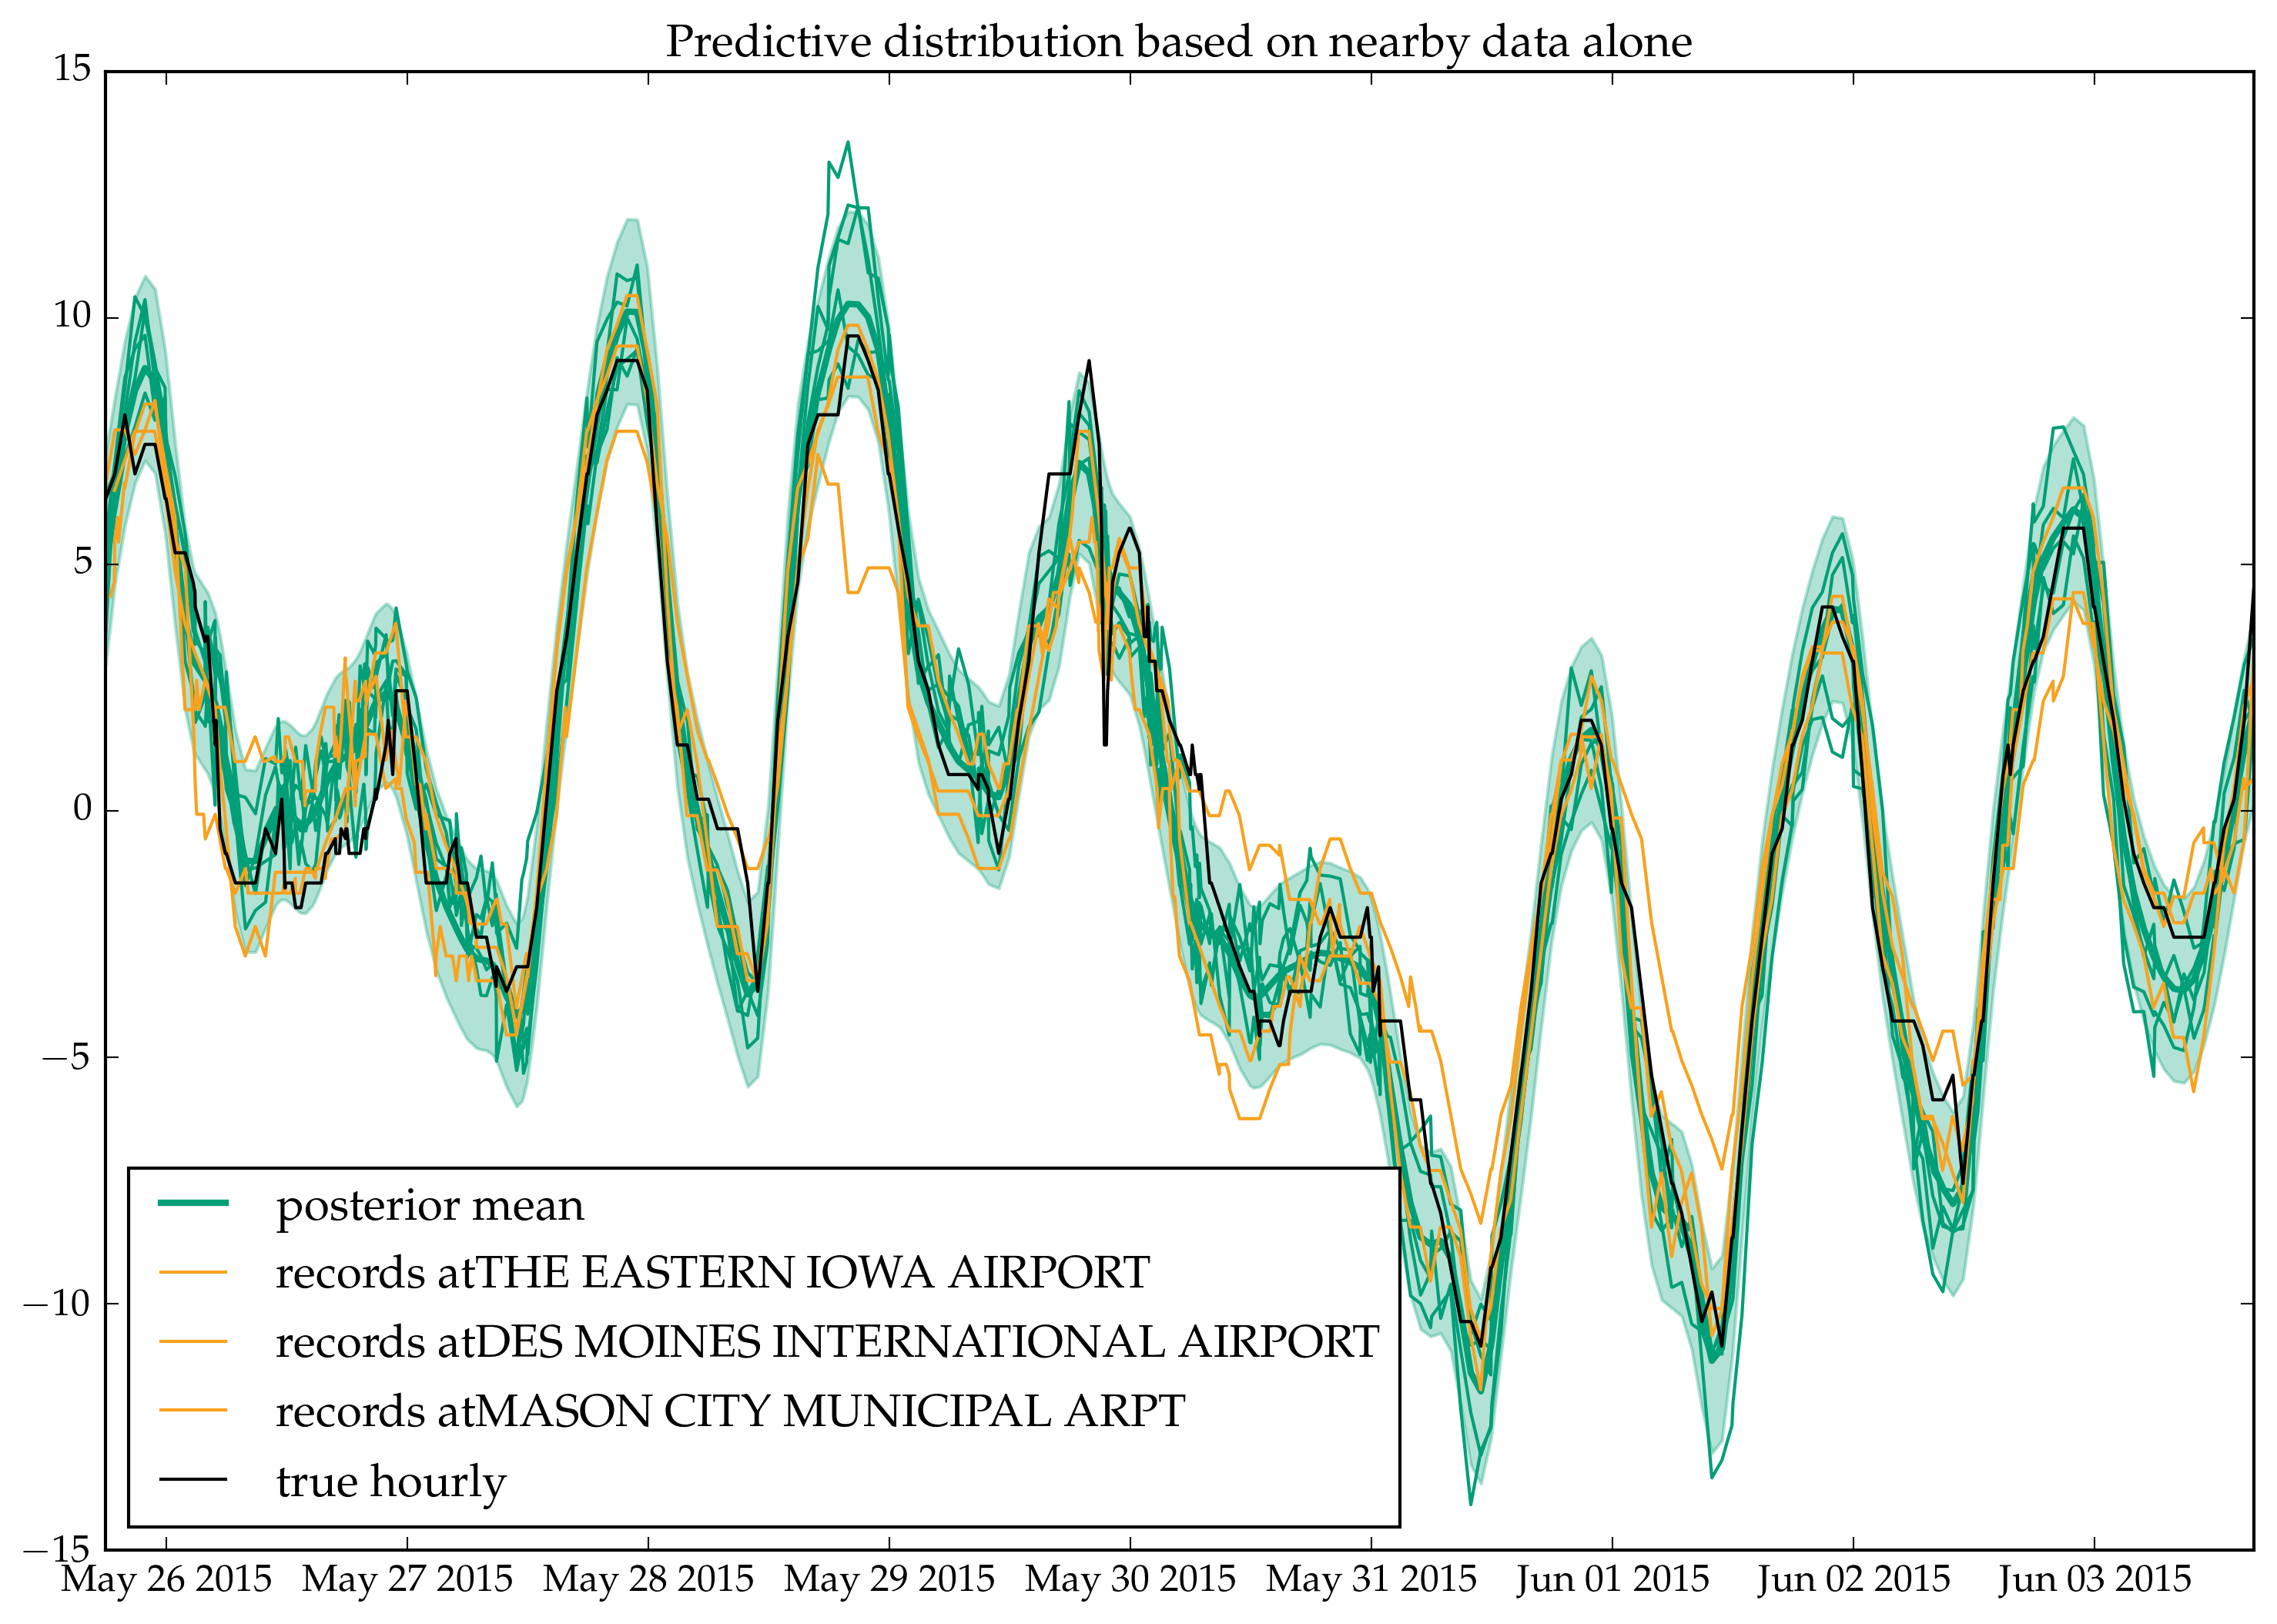
\includegraphics{figures/predictive_nearby_SEonly.png}
\caption{Predictive distribution using only nearby data and the simple product of square exponentials model. The orange lines are the measurements at nearby stations that are being used to inform the predictions. The black line is the true temperatures that have been withheld from the model, while the green line is the posterior mean of the predictions. The credible range (in green) is twice the standard deviations extracted from the diagonal entries of the posterior covariance matrix.}
\end{figure}

Once we have a spatio-temporal Gaussian process model with optimized covariance parameters, we can use it to generate predictions at the station where we aim to generate imputations based on nearby measurements.
Gaussian processes make this a closed-form procedure. We'll denote the temperatures we wish to impute as \(\T_\miss{}\) at times \(t_\miss\) and location \(\xvec_\miss\) and those observed at nearby stations as \(\T_\obs{}\), at times \(t_\obs\) and locations \(X_\obs\).
Under the spatio-temporal model, \(\T_\miss\) and \(\T_\obs\) are jointly multivariate normal, with mean zero and covariance given by \(k_{st}(\xvec,\xvec',t,t')\).
Standard results for conditioning within multivariate normals then yields

\begin{equation}
\label{eq:unconstrained_post}
\begin{split}
    \T_\miss \mid \T_\obs &\sim \normal\del{\mu_{\miss \mid \obs}, \Sigma_{\miss \mid \obs}}\,, \\
    \mu_{\miss \mid \obs} &= \E \del{\T_\miss \mid \T_\obs} \\
        &= \cov\del{\T_\miss, \T_\obs} \cov\del{\T_\obs, \T_\obs}^{-1} \T_\obs\,, \\
    \Sigma_{\miss \mid \obs} &= \var \del{\T_\miss \mid \T_\obs} \\
        &= \cov\del{\T_\miss,\T_\miss} - \cov\del{\T_\miss, \T_\obs} \cov\del{\T_\obs, \T_\obs}^{-1} \cov\del{\T_\obs, \T_\miss}\,. \\ %_
\end{split}
\end{equation}

All covariance matrices can be obtained by plugging into \(k_{st}\). For example, the \(ij\)th entry of \(\cov\del{\T_\miss, \T_\obs}\) is given by \(k_{st}(\xvec_\miss,X_\obs\sbr{j},t_\miss\sbr{i},t_\obs\sbr{j})\), where \(X_\obs\sbr{j}\) gives the spatial covariates of the \(j\)th observation, and \(t_\obs\sbr{j}\) its time.

In Figure X, we show an example of predictions obtained from this spatio-temporal model. We witheld measurements from the Waterloo Municipal Airport, and then used data from three nearby stations between May 25, 2015 and June 3, 2015 to predict the Waterloo temperatures during the same time window. This allows us to assess the quality of the predictions on this example.
    


        Our aim, however, isn't just to predict temperatures at a location with no measurements, but rather to impute hourly temperatures at a location with accurate measurements of the daily temperature extrema.
To incorporate the additional information, we can use Bayes' theorem conditionally on \(\T_\obs\)

\begin{equation}
\label{eq:posterior_constrained}
\begin{split}
    \Pr\del{\T_\miss \mid \T_\obs, \Tn, \Tx} &\propto \Pr\del{\T_\miss \mid \T_\obs} \Pr\del{\Tn, \Tx \mid \T_\miss, \T_\obs} 
\end{split}
\end{equation}

so that the posterior using nearby measurements becomes the prior for the second stage of the analysis.

In fact \(\Tn\) and \(\Tx\) act as constraints on the predictions.
For example, a \(\Tx\) record means that in the 24 hours before the measurements, the temperature reached \(\Tx\) but never exceeded it.
This means \(\Tn\) and \(\Tx\) are deterministic functions of \(\T_\miss\), and therefore

\begin{equation}
\label{eq:constraint}
\Pr\del{\Tn, \Tx \mid \T_\miss, \T_\obs} = \Pr\del{\Tn, \Tx \mid \T_\miss} = \left\{
\begin{aligned}
    1 & \,\text{ if the constraint is satisfied,} \\
    0 & \,\text{ otherwise.}
\end{aligned}
\right.
\end{equation}
    


        Conceptually, we could therefore implement a valid imputation algorithm by drawing random samples from the posterior predictive multivariate normal distribution \(\T_\miss \mid \T_\obs\) obtained from nearby measurements, and only keeping the samples that satisfy this constraint.
Unfortunately, the probability of a random draw exactly satisfying such a sharp constraint is zero, and so some tolerance would need to be introduced for overshooting or undershooting each day's \(\Tn\) and \(\Tx\) constraints.
Imputing longer periods would then require either increasing the number of samples exponentially, or further loosening this tolerance.
Ultimately, this rejection sampling strategy is therefore bound to fail.

Instead, we use the probabilistic programming language Stan to draw samples from the constrained predictive distribution.
In Stan, we specify a probabilistic data-generating process for the observed temperatures, based on parameters and latent variables with accompanying priors.
Stan then uses a Hamiltonian Monte Carlo (HMC) algorithm to draw sample from the posterior distribution for the parameters and latent variables.
In our case, the observations are the daily maxima and minima, the only parameter is the average temperature at the station of interest \(\mu_\miss\), and the latent variables are the missing unobserved hourly temperatures \(\T_\miss\).
    


        To summarize, the probabilistic model that we wish to draw posterior imputations of \(\T_\miss\) from is given in \eqref{eq:idealmodel}.

\begin{equation}
\label{eq:idealmodel}
\begin{aligned}
    \mu_\miss &\sim \normal\del{0,100} & \text{ (vague prior on mean temperature)} \\
    f_\miss &\sim \normal\del{\mu_{\miss \mid \obs}, \Sigma_{\miss \mid \obs}} & \text{ (posterior from $\T_\obs$ becomes prior)} \\
    \T_\miss &= \mu_\miss + f_\miss \\
    \Tx\sbr{\iday} &= \max_{i \in \dayset{\iday}}\cbr{ \T_{\miss,i}} & \text{ (observe maximum in 24hr window)}\\
    \Tn\sbr{\iday} &= \min_{i \in \dayset{\iday}}\cbr{ \T_{\miss,i}} & \text{ (observe minimum in 24hr window)}\\
    \dayset{\iday} &= \cbr{i : \iday-1+\frac{\hour}{24} \lt t_{\miss,i} \le \iday + \frac{\hour}{24}} & \text{ (indices of times in the 24hr window)}
\end{aligned}
\end{equation}
    


        The problem caused by the sharp constraint remains. At each step of the Markov chain, a proposal is made for \(T_\miss\). If the daily maxima and minima of this proposal coincide exactly with the measurements, then its posterior probability is finite. Otherwise it is exactly zero, with gradient also zero. HMC works by exploiting the gradient of the posterior, and therefore fails to converge in this situation, for reasons similar to the failure of the naive rejection sampler.

\begin{figure}
\centering
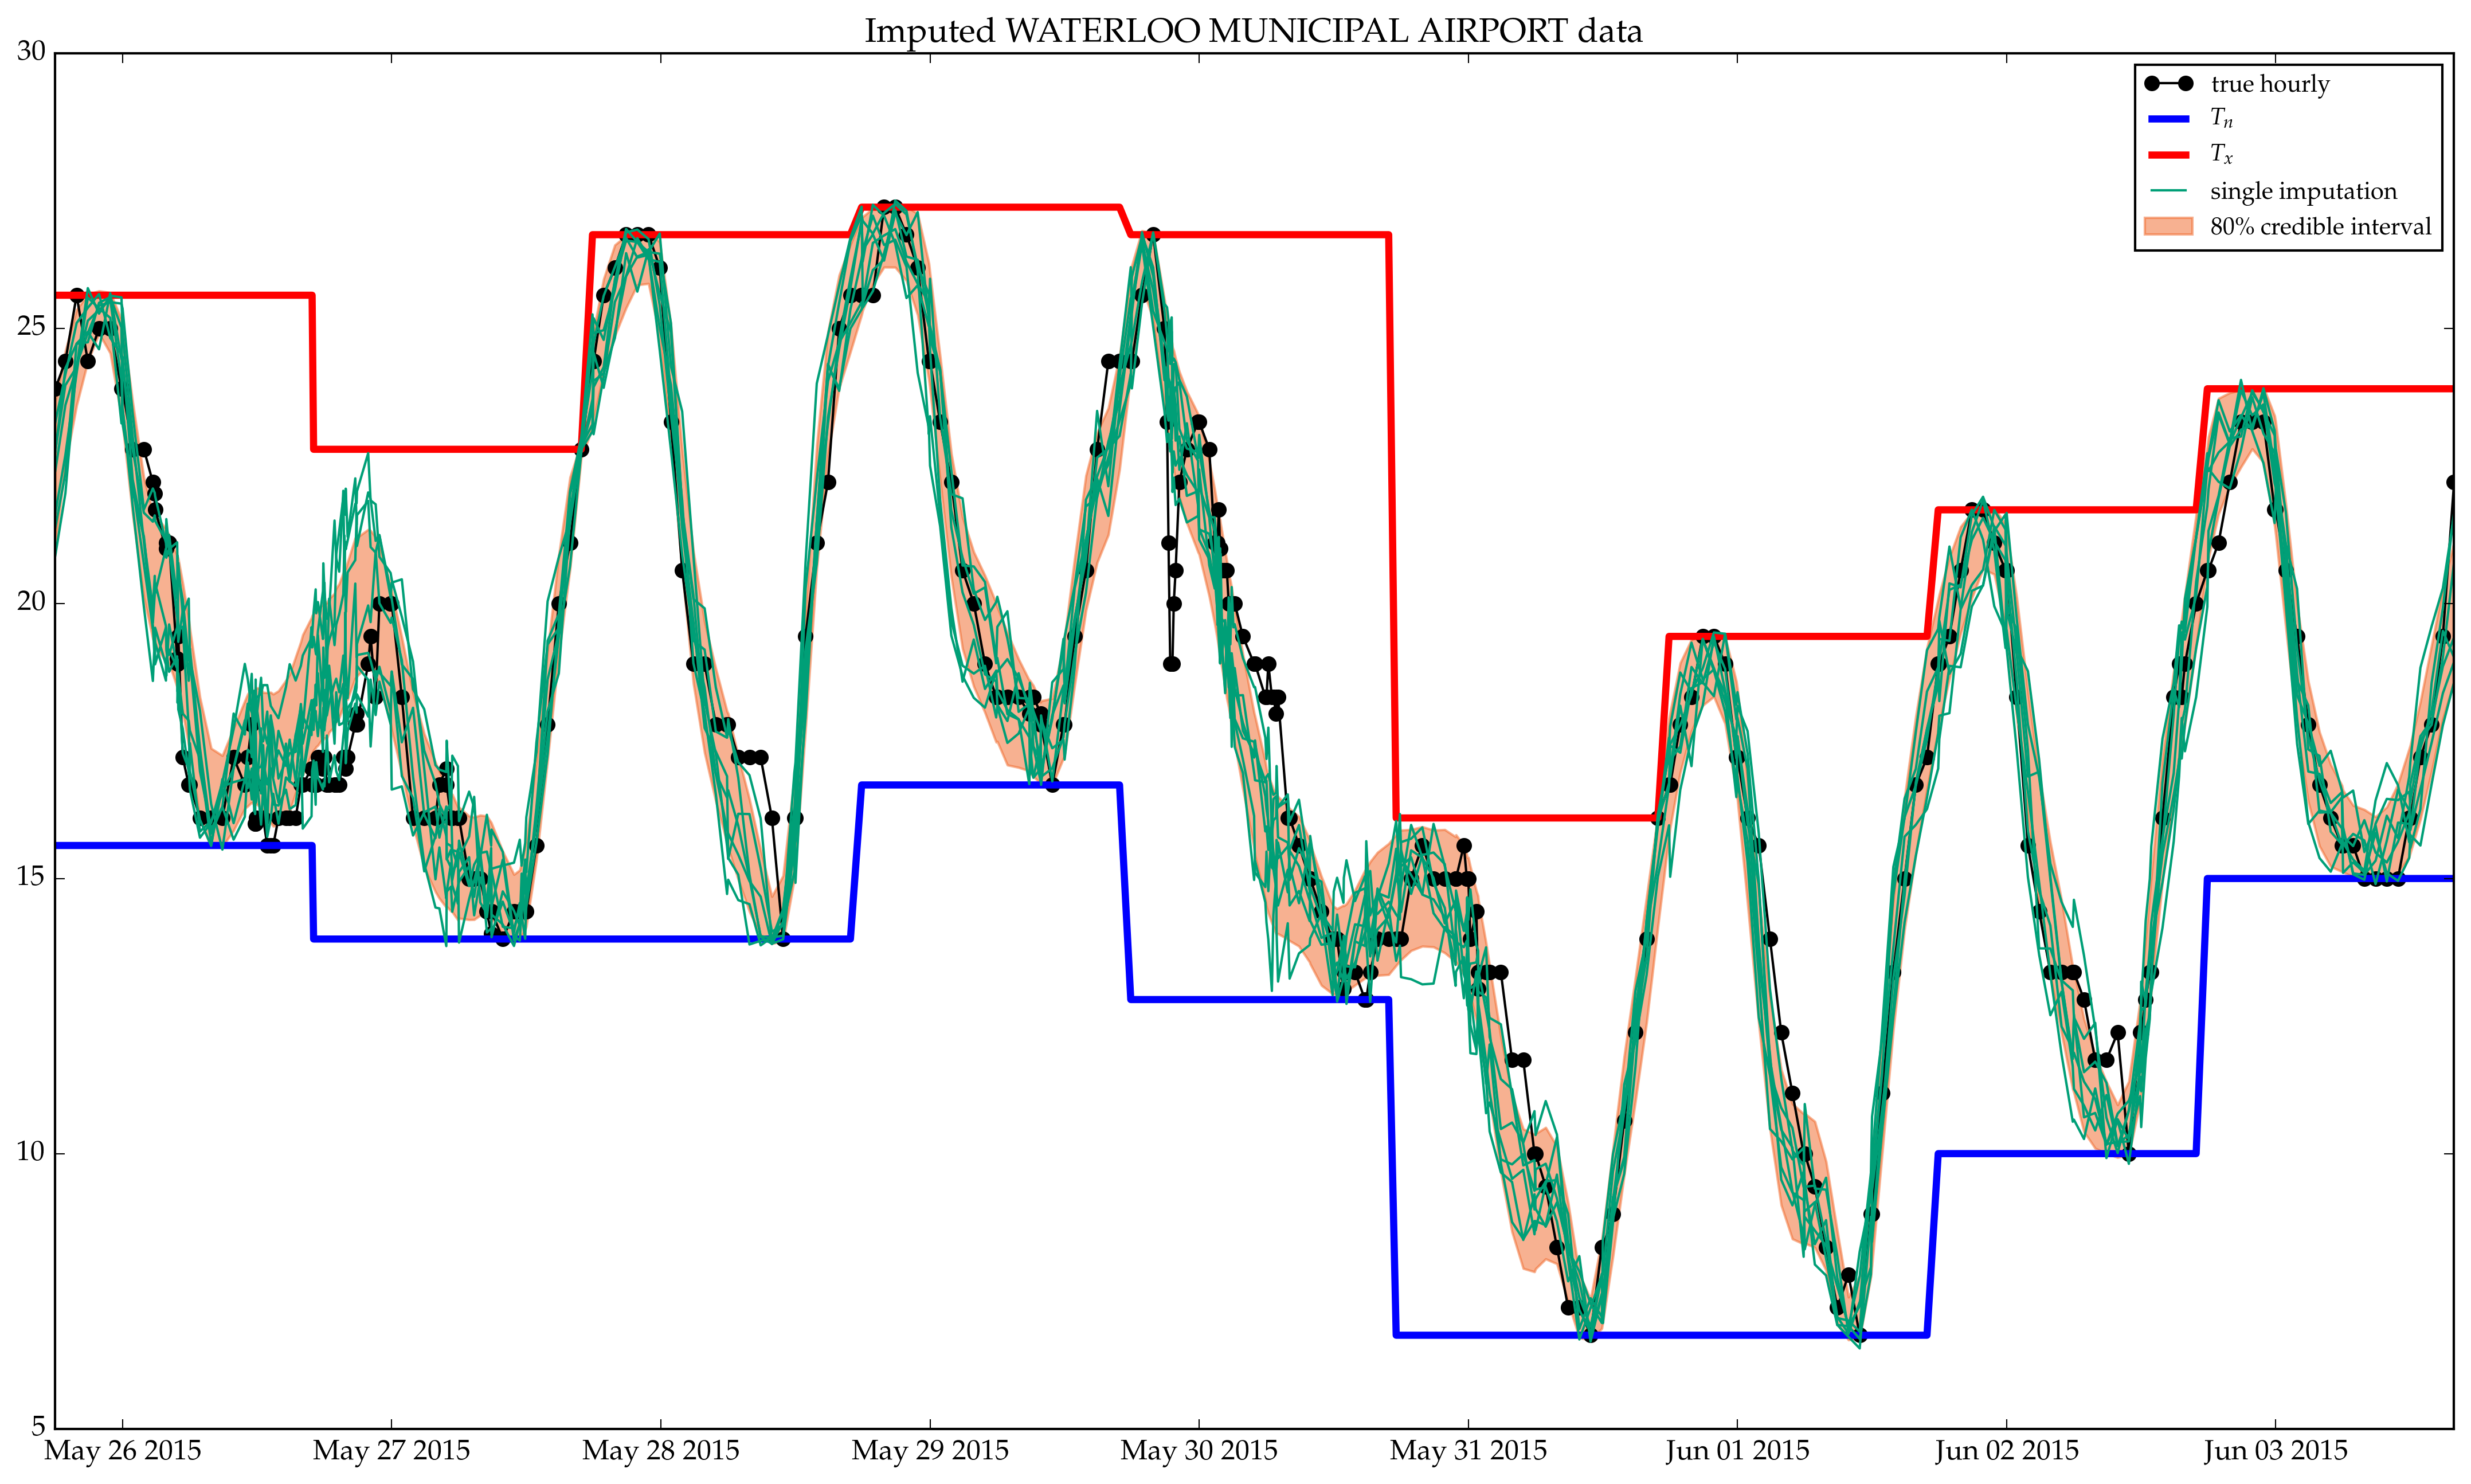
\includegraphics{figures/imputations_SEonly.png}
\caption{Imputations at Waterloo Airport from May 25, 2015 to June 3, 2015}
\end{figure}

We can rescue the algorithm by replacing the \(\max\) and \(\min\) functions with the \(\softmax\) and \(\softmin\) functions, which take real inputs \(x_1, \ldots, x_p\) and a sharpness parameter \(k\) and return

\begin{equation}
\begin{split}
    \softmax\del{x_1, \ldots, x_p ; k} &= \frac{1}{k} \log\del{\sum_{i=1}^p e^{kx_i}} \\
    \softmin\del{x_1, \ldots, x_p ; k} &= -\softmax\del{-x_1, \ldots, -x_p; k}
\end{split}
\end{equation}

As \(k \rightarrow \infty\), \(\softmax\) becomes the maximum, and \(\softmin\) becomes the minimum.
Lower values of \(k\) give close approximations. When \(\softmax\) replaces \(\max\) and \(\softmin\) replaces \(\min\), there is a small price in precision due to the approximation, but there is a huge computational benefit: gradients are now available.
Furthermore, by adding a small amount of white noise with variance \(\sigma_\epsilon\) to the \(\Tx\) and \(\Tn\) measurements, we ensure that the posterior doesn't go abruptly to zero when the conditions aren't met exactly.
These modifications make HMC a viable algorithm to efficiently draw samples from the constrained posterior.
Setting \(k\) and \(\sigma_\epsilon\) is a compromise between exactness and efficiency;
we found \(k=10\) and \(\sigma_\epsilon=0.1\) to perform well.
The modified model is given below, and approximates our ideal model \eqref{eq:idealmodel}.

\begin{equation}
\label{eq:smoothed_model}
\begin{split}
    \mu_\miss &\sim \normal\del{0,100} \\
    f_\miss &\sim \normal\del{\mu_{\miss \mid \obs}, \Sigma_{\miss \mid \obs}} \\
    T_\miss &= \mu_\miss + f_\miss \\
    \Tx\sbr{\iday} &\sim \normal\del{\softmax_{i \in \dayset{\iday}} \cbr{ T_{\miss,i}; k=10}, 0.1^2} \\
    \Tn\sbr{\iday} &\sim \normal\del{\softmin_{i \in \dayset{\iday}} \cbr{ T_{\miss,i}; k=10}, 0.1^2}
\end{split}
\end{equation}

Example imputations from this procedure are shown in Figure X.
From May 25, 2015 to June 3, 2015, hourly temperatures are imputed at Waterloo Airport, using the hourly temperature measurements from nearby stations to inform the course of the temperatures, and using the daily minima and maxima ``measurements'' to constrain the imputed temperatures, and to infer the mean.
Because we actually have hourly data for Waterloo, yet only fed our algorithm a reduction of this data to daily extremes, we can also plot the hidden temperatures, and see how faithfully the imputations reproduce them.
We see that the imputations indeed track the true measurements very closely.
The error bars satisfyingly narrow and widen in accordance to the amount of information available at each moments.
On May 27th, we can see that the imputations capture the fact that the \(\Tx\) record \emph{could} have been set early in the measurement window, but more likely at its very end.
    


        \section{Model diagnostics}\label{model-diagnostics}

\subsection{Variogram}\label{variogram}

We can visually inspect our model by plotting temporal and spatial semi-variograms. The semi-variogram of a stationary spatio-temporal function \(Y(\xvec,t)\) is a function of the spatial lag \(\hvec\) and the temporal lag \(r\)

\begin{equation}
    \gamma\del{\hvec,r} = \frac{1}{2} \E\sbr{\del{Y\del{\xvec,t}-Y\del{\xvec+\hvec,t+r}}^2} = \var\del{ Y\del{\xvec,t}} - \cov\del{ \del{Y\del{\xvec,t}} , Y\del{\xvec+\hvec,t+r}}\,.
\end{equation}

For a Gaussian Process model, with a stationary kernel \(k(\hvec,r)=k(\xvec,\xvec+\hvec,t,t+r)\) this can be expressed in terms of the observation noise \(\sigman\) and kernel function \(k(\cdot,\cdot)\), as

\begin{equation}
    \label{eq:gp_variogram}
    \gamma\del{\hvec,r} = \sigman^2 + k\del{0,0} - k(\hvec,r)\,.
\end{equation}

From the data, the semi-variogram can also be estimated empirically, be averaging the square differences of any two observations that are separated by \(\hvec\) in space, and \(r\) in time (or, in practice, within half a bin width of \(\hvec\) and \(r\)). By comparing the empirical variogram to the variogram of our fitted \(\GP\) model, we obtain a visual diagnosis of the model.

In our Iowa example, there are only four possible locations. For each location, we plot the empirical temporal variogram \(\hat\gamma\del{0,r}\). For any pair of stations separated by \(\hvec\) (fixed), we can also plot \(\hat\gamma\del{\hvec,r}\). We then overlay the model's semi-variogram obtained through equation \eqref{eq:gp_variogram}, resulting in Figure~\ref{fig:spatial_variogram}.

\begin{figure}
\centering
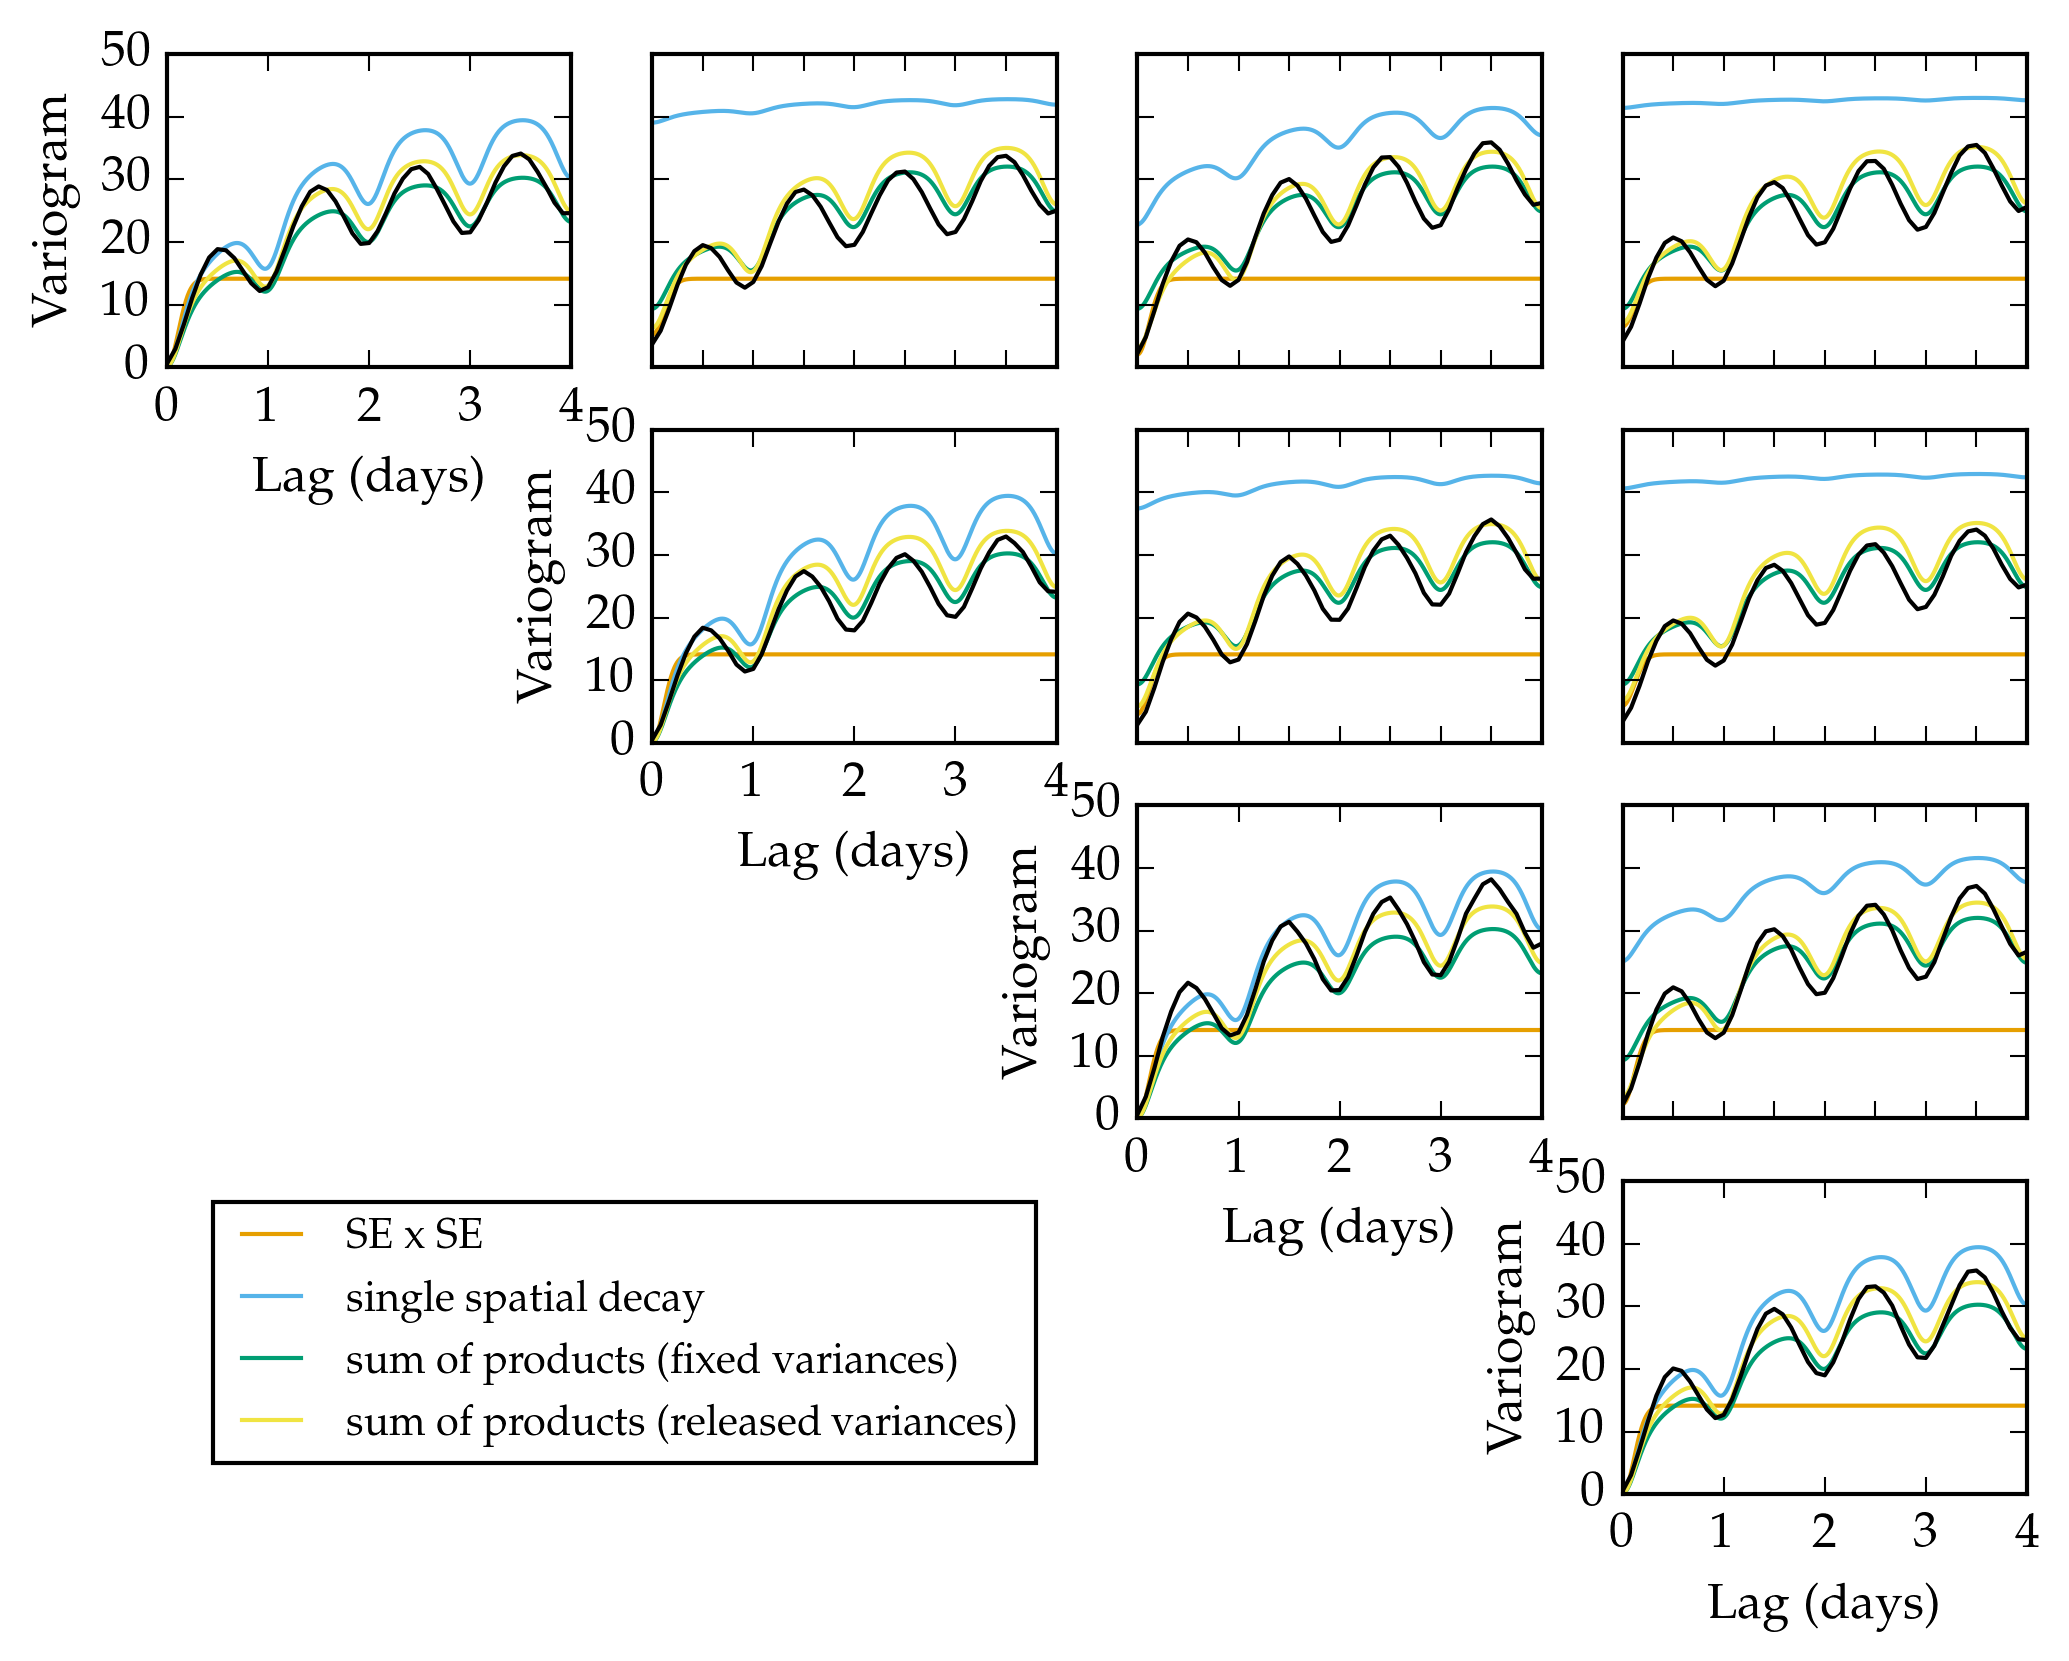
\includegraphics{figures/spatial_variogram.png}
\caption{\label{fig:spatial_variogram} Semi-variogram}
\end{figure}
    


        We notice that the variogram of the simple \texttt{SExSE} model tracks the empirical variogram well at short lags, but fails to capture the diurnal cycle, and the fit degrades at long lag. We attempt to improve the model in section \ref{sec:improving_model}.
    


        \subsection{Error and expected error}\label{error-and-expected-error}

The variogram gives us a visual diagnostic of the overall model fit. To quantify the model's predictive ability in the Iowa example, we compare the posterior mean temperature to the withheld truth, and obtain the empirical mean squared error as

\begin{equation}
    \label{eq:mse}
    \mse\del{\error \mid \T_\obs,\Tx,\Tn} = \frac{1}{N} \sum_{i=1}^N \sbr{\E\del{\T_{\miss,i} \mid \T_\obs,\Tx,\Tn} - \T_{\miss,i}}^2\,.
\end{equation}

This equation is for the final predictions obtained using nearby hourly temperatures and local daily maxima and minima.
A similar diagnostic can be computed for the intermediary predictions, which exclude the local \(\Tx\) and \(\Tn\) information.
At that stage, we are not concerned with any overall bias in the predicted temperatures, so we instead compute the sample variance of the errors as

\begin{equation}
    \label{eq:varerr}
    \var\del{\error \mid \T_\obs} = \var_i \cbr{\E\del{\T_{\miss,i} \mid \T_\obs} - \T_{\miss,i}}\,.
\end{equation}

\begin{longtable}[]{@{}llllll@{}}
\toprule
Model & Log Likelihood & Var(err) & \(\E\)(Var(err)) & MSE(err) & \(\E\)(MSE(err))\tabularnewline
\midrule
\endhead
SE x SE & -55,614 & 1.589 & 0.875 & 1.104 & 0.614\tabularnewline
SExSE + diurnal & -54,472 & 1.633 & 0.974 & 1.137 & 0.697\tabularnewline
Sum of products, fixed variance & -48,589 & 4.991 & 8.791 & &\tabularnewline
SoP, fixed temporal, free var & -47,082 & 1.314 & 2.321 & 1.150 & 0.897\tabularnewline
SoP, completely free & -46,184 & 1.423 & 1.765 & 1.152 & 0.950\tabularnewline
SoP, simpler & -45,945 & 1.319 & 1.190 & 1.069 & 0.823\tabularnewline
\bottomrule
\end{longtable}

For our purposes, it isn't sufficient for the spatio-temporal model to yield good predictions; we also require a good estimate of its own accuracy.
We estimate the expected MSE and predictive variance by sampling \(K\) random draws \(\T^k_\miss\) from the posterior distribution, again conditioned firstly on just \(\T_\obs\) after fitting the spatio-temporal Gaussian process model, and then additionally on \(\T_\obs\), \(\Tx\) and \(\Tn\) after incorporating the local data using Stan.
The draws are obtained from the posterior multivariate normal distribution in the first case, and the MCMC samples obtained through Stan in the second case.
We then evaluate the variance or MSE between the samples and the posterior mean as

\begin{equation}
\begin{split}
    \E \del{\var\del{\error \mid \T_\obs}} &\approx \frac{1}{K} \sum_{k=1}^K \var_i \cbr{\T^{(k)}_{\miss,i} - \E\del{\T_{\miss,i} \mid \T_\obs}} \\
    \E \del{\mse\del{\error \mid \T_\obs,\Tx,\Tn}} &\approx \frac{1}{K} \sum_{k=1}^K \mse_i \cbr{\T^{(k)}_{\miss,i} - \E\del{\T_{\miss,i} \mid \T_\obs,\Tx,\Tn}} \\
\end{split}
\end{equation}

When evaluating models, we want the errors to be small, and so the empirical error variance and MSE to be low. A well-calibrated model should also have the expected error variances \(\E \del{\var\del{\error \mid \cdot}}\) close to their empirical values.

These diagnostics for our first spatio-temporal model, the product of squared exponentials, are found in the first row of Table X. The empirical error variance using only nearby measurements is already fairly low, with typical errors of order \(\sqrt{1.589}=1.26\,\degreeC\). Incorporating the local measurements reduces it further to \(\sqrt{1.104}=1.05\,\degreeC\). However, the model is overly optimistic, and the expected errors underestimate the true errors.
    


        \section{Improving model}\label{improving-model}
    

\label{sec:improving_model}
        In this section, we develop more sophisticated Gaussian process models than the simple product of squared exponential kernels. We then assess whether these models improve the variogram and the predictive diagnostic measures that we developed in the previous sections.

The most salient feature of the empirical variogram that isn't captured by the \texttt{SExSE} model is the oscillation with a 24-hour period. It is intuitively obvious that the diurnal cycle induces this periodic covariance, and that our model should be improved by incorporating this feature. Gaussian process models allow for periodic components of the covariance, for example the periodic squared exponential kernel, which we will use with a 24-hour period

\begin{equation}
    k_{24}(t,t') = \sigma_{24}^2 \exp\sbr{ - \frac{2}{\ell_{24}^2} \sin^2\del{
        \pi \frac{t-t'}{\text{24 hrs}} 
        }}\,.
\end{equation}

We modify the spatiotemporal model by adding this diurnal component to it, with its own spatial decay kernel \(k_{space24}\) (with the same specification as \(k_{space}\) in \eqref{eq:kspace}).

\begin{equation}
    \kdiurn(\xvec,\xvec',t,t') = k_{time}(t,t') \cdot k_{space}(\xvec, \xvec') 
        + k_{24}(t,t') \cdot k_{space24}(\xvec, \xvec')
        + k_\mu(\xvec, \xvec') 
        \,.
\end{equation}
    


        We also develop a more complex model, which breaks up \(k_{time}\) into short-term, medium-term and long-term correlation components, each with their own spatial decay.

\begin{equation}
\begin{aligned}
    \ksumprod(\xvec,\xvec',t,t') &= 
           k_{time1}(t,t') \cdot k_{space1}(\xvec, \xvec')  &\text{(short-term variation)} \\
        &+ k_{time2}(t,t') \cdot k_{space2}(\xvec, \xvec')  &\text{(medium-term variation)} \\
        &+ k_{time3}(t,t') \cdot k_{space3}(\xvec, \xvec')  &\text{(long-term variation)} \\
        &+ k_{24}(t,t') \cdot k_{space24}(\xvec, \xvec') &\text{(diurnal cycle)} \\
        &+ k_\mu(\xvec, \xvec') &\text{(station mean)}
\end{aligned}
\end{equation}

Each of \(k_{time1}\), \(k_{time2}\), and \(k_{time3}\), is a rational quadratic kernel

\begin{equation}
    k_{RQ}(t,t') = \sigma^2 \del{1 + \frac{\del{t-t'}^2}{2\alpha\ell^2} }^{-\alpha}
\end{equation}

which is accompanied by its spatial decay kernel, specified as a squared exponential covariance.
This more complicated kernel therefore has \(3 \times 3 \times 2 + 2 \times 2 = 22\) free parameters, in addition to the noise parameter \(\sigman^2\).

We now have three competing Gaussian process models, with covariance functions \(\kSESE\), \(\kdiurn\), and \(\ksumprod\) respectively. We can compare them in three ways. Firstly, the marginal log-likelihood is the quantity maximized by the parameter fitting procedure in \eqref{eq:optimization}. The maximized log-likelihood can be found in the second column of Table~XX, and we see that the more complex models indeed yield a much higher log-likelihood, promising a better model fit which should yield better predictions. Secondly, we compare the variance of the error in the predicted temperatures specified in \eqref{eq:varerr} when withholding all the data from a test station. Averaged over all of 2015, this is given in the third column, and shows more mixed results. The diurnal model \(\kdiurn\) performs worse than the simple \(\kSESE\) model, and \(\ksumprod\) only yields a small improvement.
Thirdly, we can reintroduce the daily minima and maxima from the withheld station, and compare the mean squared error specified in \eqref{eq:mse} for predictions at the test station. Results in the fifth column show even more modest improvements for the more complex models.

We interpret these results as a reminder that predictions using Gaussian process are sensitive to model specification when extrapolating, but fairly insensitive to the model when interpolating {[}cite?{]}. Since our imputations interpolate the temperatures from nearby stations, further aided by the constraints imposed by the daily \(\Tn\) and \(\Tx\) measurements, the choice of model does not have a large impact on the performance of our procedure. This insensitivity can be seen as reassuring, as it (to an extent) reduces our need to worry about the incorrectness of our model.
    


        \section{Analysis}\label{analysis}

\begin{itemize}
\tightlist
\item
  show imputations on interesting days
\item
  show imputations can capture two possible explanations for a measurement
\item
  discuss possibility of inferring measurement time
\end{itemize}
    


        \section{Inference on measurement hour}\label{inference-on-measurement-hour}

Our analysis so far has focused on the case where the hour of measurement \(\hour\) is known in advance.
This is an unrealistic assumption in practice, and so inference on \(\hour\) is a desirable feature.
It is conceptually straightforward to modify \eqref{eq:smoothed_model} with a uniform prior on \(\hour\).
However, because we obtain our imputations in ten-day windows, in most windows precise information about \(\hour\) will not be available, as moving the measurement time one hour earlier or later rarely affects the measured \(\Tn\) and \(\Tx\).
Furthermore, \(\hour\) affects which observations are attributed to each day's measurements.
This effect is discontinuous (observations suddenly jump from one day to the next) and non-differentiable, and so Hamiltonian Monte Carlo becomes unviable.
This issue is similar to that caused by the non-differentiability of the minimum and maximum functions.
We therefore do not consider the introduction of a uniform prior on \(\hour\) in Stan to be feasible.

Our procedure allows us to obtain imputation samples of \(\T_\miss\) conditional on \(\T_\obs,\Tn,\Tx\) and \(\hour\).
If we do so for \(\hour=1,2,\ldots,24\), is there information available in these samples to infer \(\hour\)?
We will examine sample imputations to answer this question.
Figure~\ref{fig:measure_hour_example} shows mean imputation for temperatures over nine days starting on February~27, 2015. The orange line is the mean using only nearby temperatures (shifted by a constant to match the true temperatures), while the green line is additionally conditional on \(\Tn\) and \(\Tx\); the true temperatures are shown in grey.
The top plot shows the imputation under the correct daily measurement time (17 UTC), while the bottom plot is under an incorrect measurement time (5 UTC).
The first unsurprising observation is that assuming an incorrect measurement time can lead to wildly inaccurate imputations.
But we then also notice that assuming the wrong time also causes the mean constrained imputation to depart further from the unconstrained imputation
(that is, the green and orange lines are further apart).
This can be interpreted as an indication of an incompatibility between \(\T_\obs\) and the daily extremes, caused by assuming the wrong \(\hour\).
To quantify this discrepancy, we propose to calculate the probability of the mean constrained imputation under the unconstrained posterior given by \(\eqref{eq:unconstrained_post}\):

\begin{equation}
\begin{split}
    \mu\del{\hour} &\equiv \E\del{ \T_\miss \mid \T_\obs, \Tn, \Tx, \hour } \text{ (the mean imputed temperature), }\\
    \discrepancy_\hour &\equiv \Pr\del{ \T_\miss = \mu\del{\hour} \mid \T_\obs }\,.
\end{split}
\end{equation}

Our intuition is that \(\discrepancy_\hour\) will drop sharply when the wrong \(\hour\) is assumed,
and we may be able to infer the true \(\hour\) by maximizing \(\discrepancy_\hour\).
    


        \begin{figure}
\centering
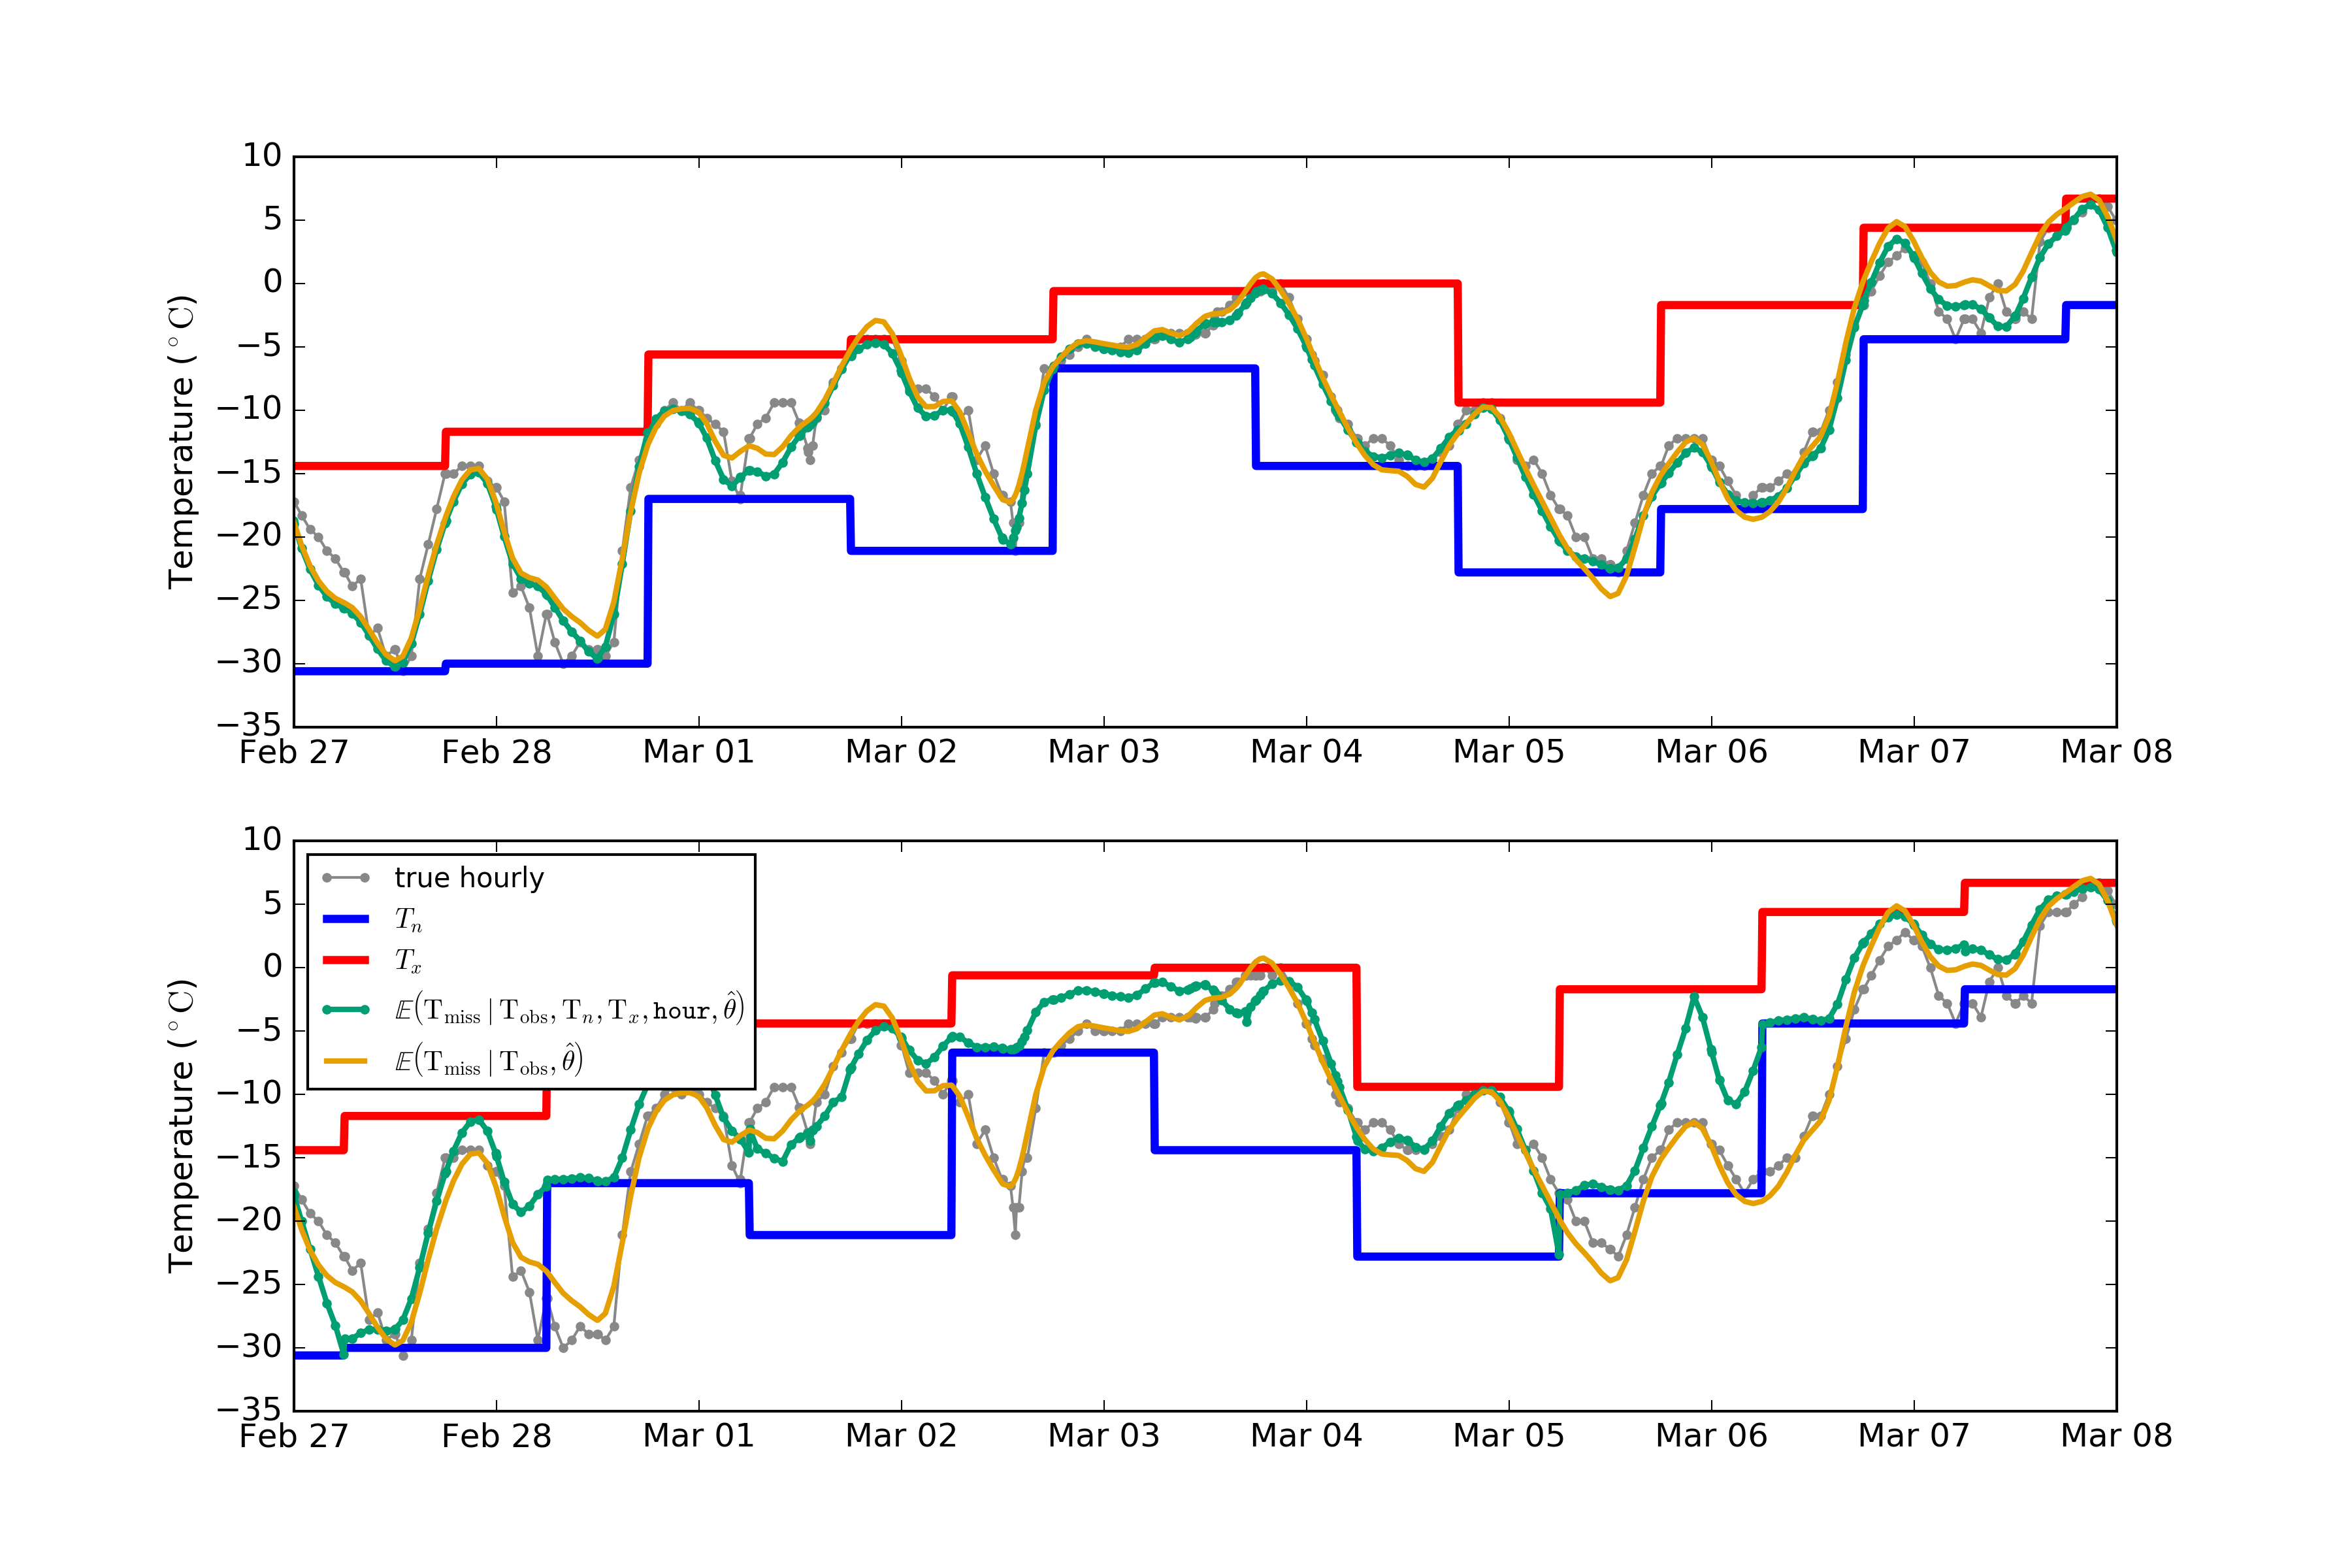
\includegraphics{figures/measure_hour_example.png}
\caption{\label{fig:measure_hour_example} A sample window showing constrained and unconstrained imputations assuming (top) the correct measurement hour (17 UTC), and (bottom) the wrong measurement hour (5 UTC). Assuming the wrong measurement time drives the constrained mean imputation away from the unconstrained mean imputation.}
\end{figure}
    


        \begin{figure}
\centering
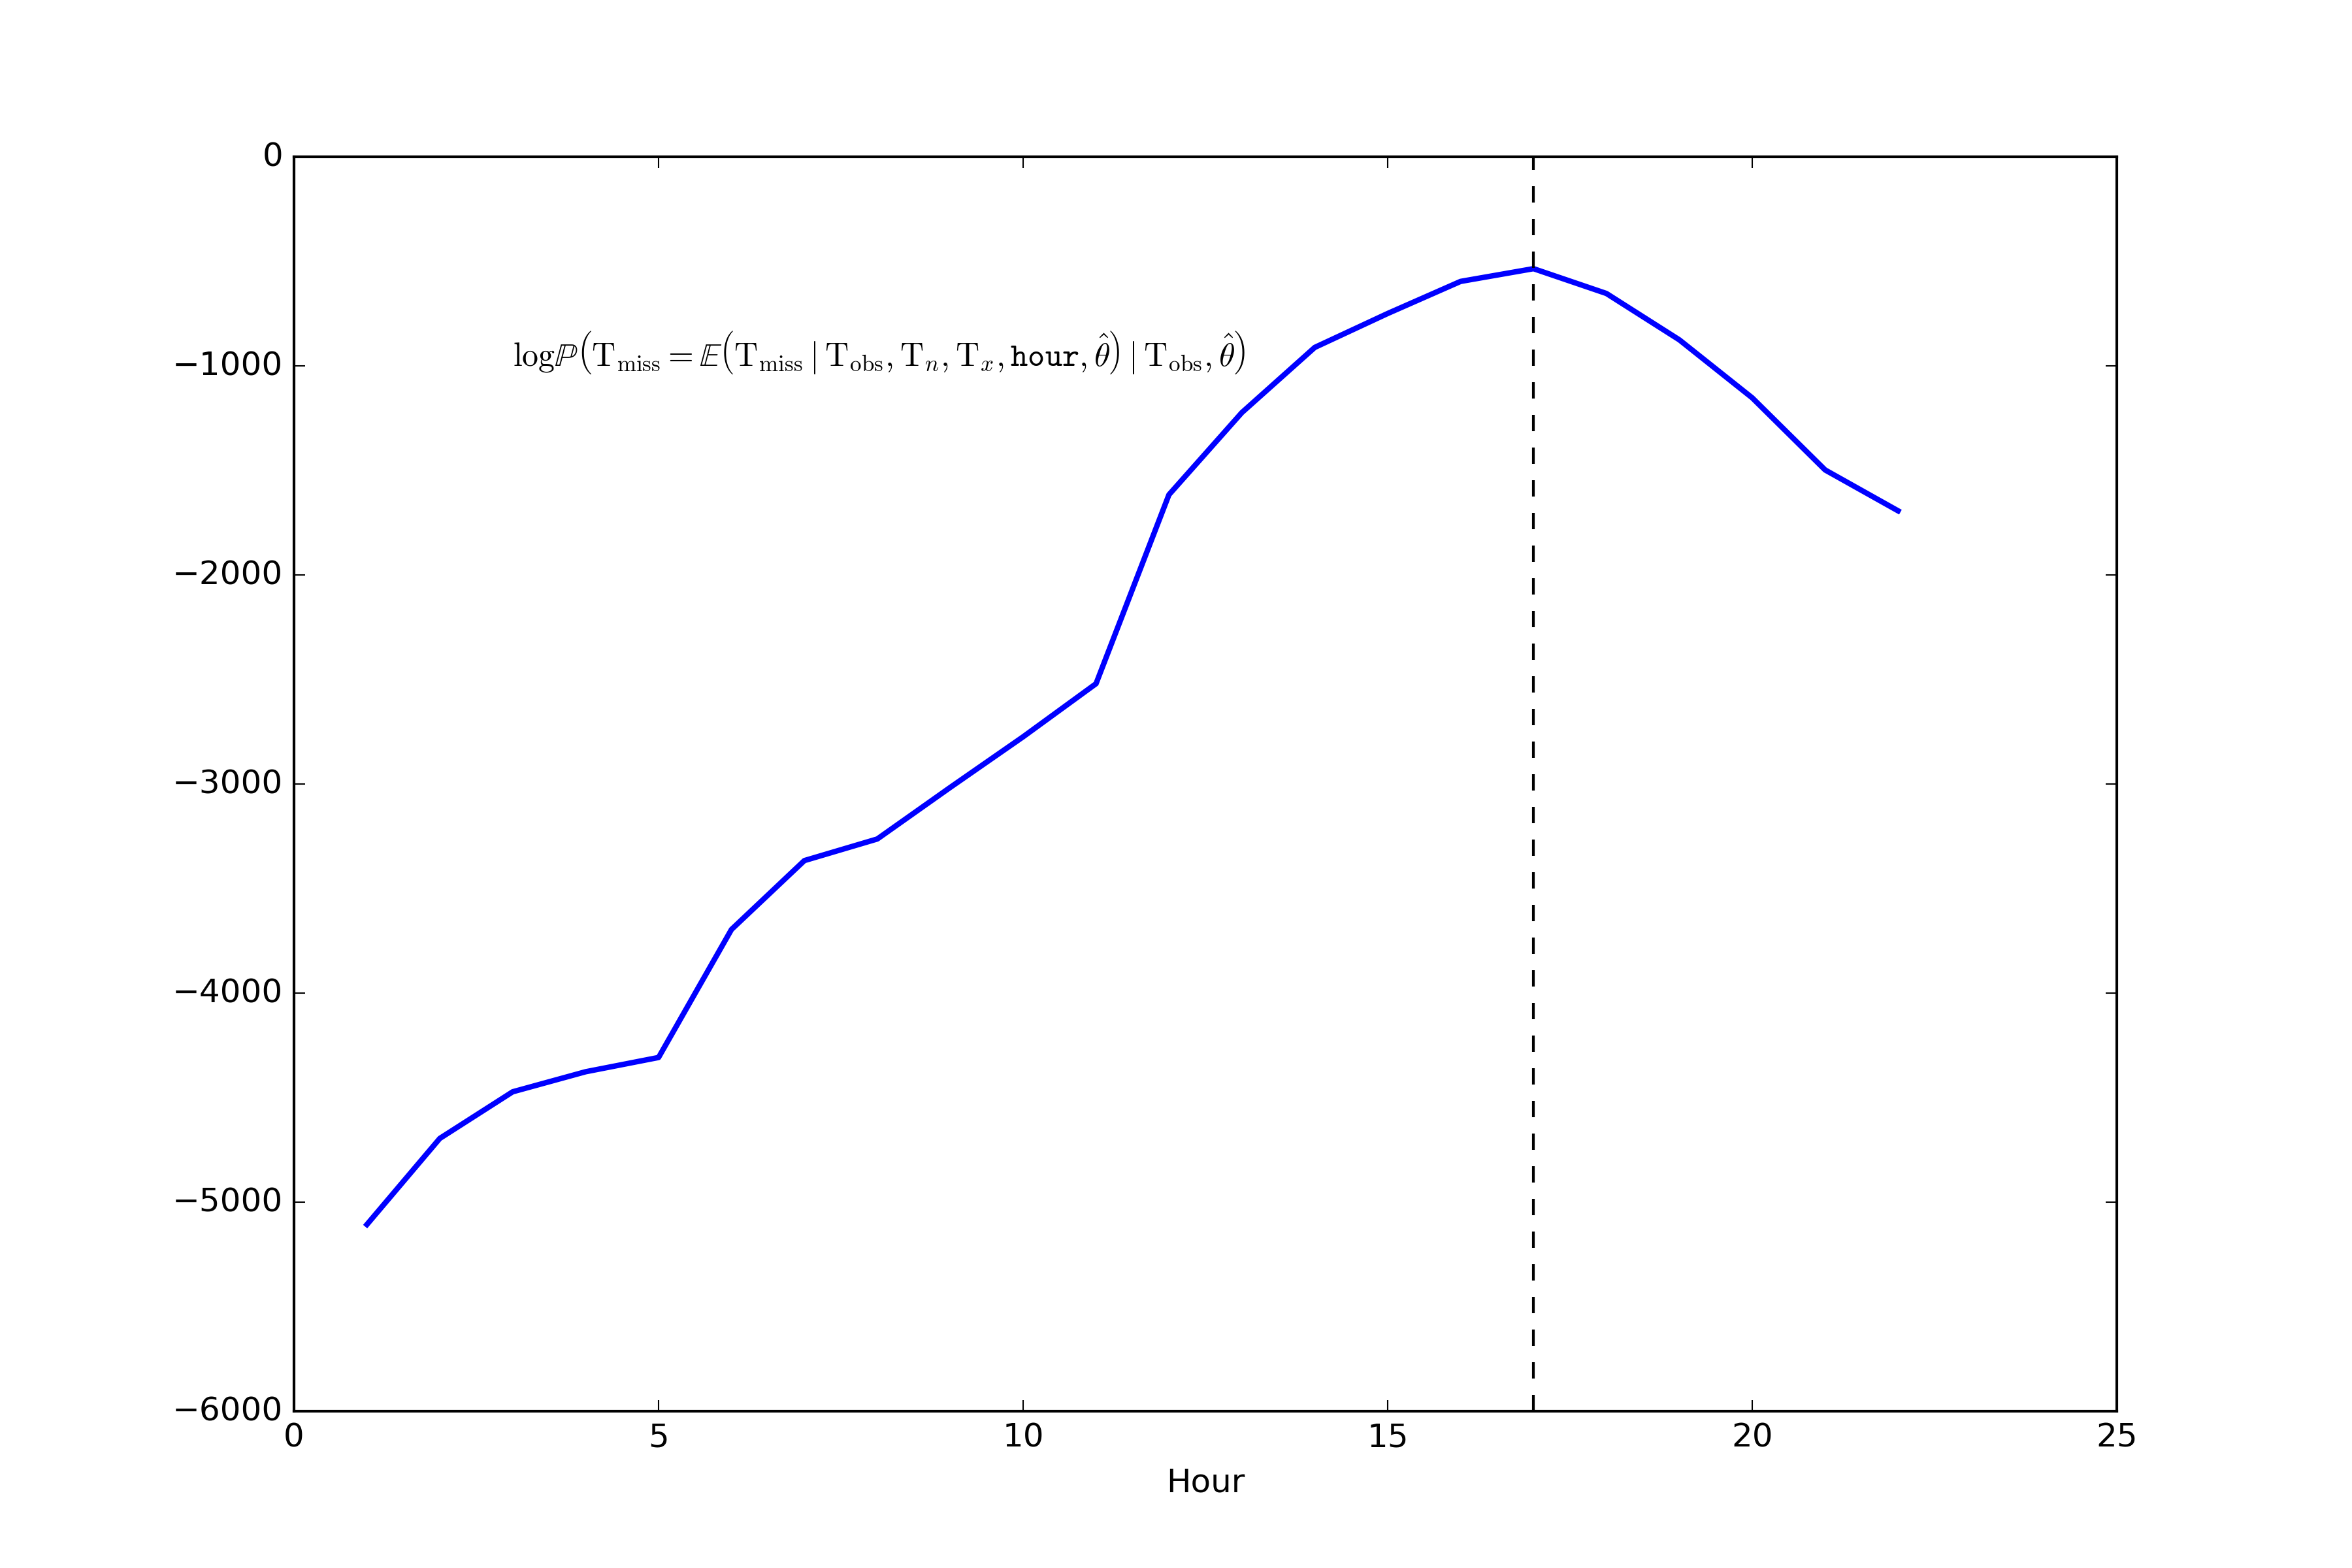
\includegraphics{figures/hr_inference.png}
\caption{\label{fig:hr_inference} Discrepancy measure for imputations of temperatures at Waterloo Municipal Airport assuming measurement hours \(\hour=1,2,\ldots,24\). The true hour of measurement is 17, and obtains the highest \(\delta_\hour\).}
\end{figure}
    


        Fortuitously, our discrepancy measure \(\discrepancy_\hour\) also admits a Bayesian interpretation: is is proportional to the marginal likelihood of \(\hour\) under (admittedly fanciful) approximating assumptions.
Ideally, we would evaluate the marginal likelihood \(\Pr\del{\Tn,\Tx \mid \T_\obs, \hour}\), and then appeal to Bayes theorem to obtain a posterior on \(\hour\)

\begin{equation}
    \Pr\del{\hour \mid \Tn, \Tx, \T_\obs } \propto \Pr\del{\Tn,\Tx \mid \T_\obs, \hour} \Pr\del{\hour}\,.
\end{equation}

However, marginal likelihoods are notoriously difficult to estimate from posterior samples {[}cite? Raftery 1994?{]}.
The marginal likelihood is the normalizing constant for the posterior \eqref{eq:posterior_constrained} of \(\T_\miss\), and therefore for any \(\T_\miss\)

\begin{equation}
\begin{split}
    \Pr\del{\Tn,\Tx \mid \T_\obs, \hour} &= \frac{
        \Pr\del{\Tn,\Tx \mid \T_\miss, \cancel{\T_\obs}, \cancel{\hour}} 
        \Pr\del{\T_\miss \mid \T_\obs, \cancel{\hour}}
    } { 
        \Pr\del{\T_\miss \mid \Tn,\Tx,\T_\obs, \hour}
    }\,.
\end{split}
\end{equation}

The first term in the numerator is either one or zero, as discussed near equation \eqref{eq:constraint}.
If we assume the constraint is satisfied,
pick \(\T_\miss = \mu\del{\hour}\),
and assume that the posterior density evaluated at its mean
does not depend heavily on the time of measurement,
we obtain that the marginal likelihood is proportional to \(\discrepancy_\hour\).
Both assumptions are fanciful: the posterior mean generally will violate the constraint imposed by \(\Tn\) and \(\Tx\), and therefore the likelihood \(\Pr\del{\Tn,\Tx \mid \T_\miss}\) should in fact be zero.
Furthermore, there is no reason to think the posterior density at the posterior mean does not depend on \(\hour\), but we might reasonably hope that the wrongness of this assumption does not overwhelm the signal contained in \(\discrepancy_\hour\).
This reasoning at least confirms that \(\discrepancy_\hour\) captures information about the likelihood of \(\hour\), and that once renormalized it can be loosely interpreted as a posterior probability under a uniform prior.
    



    % Add a bibliography block to the postdoc
    
    
\bibliographystyle{ametsoc2014}
\bibliography{ref}

    
    \end{document}
